\chapter{Πειράματα}
Προκειμένου να αξιολογηθεί η απόδοση του προτεινόμενου περιγραφέα, οργανώθηκαν και εκτελέστηκαν πειράματα ταξινόμησης εικόνων. Για την εξαγωγή των τοπικών χαρακτηριστικών έγινε χρήση της προτεινόμενης αναπαράστασης και, προκειμένου να μπορεί να γίνει κάποια σύγκριση, του αλγόριθμου SIFT (Κεφ \ref{subsec:sift}). Έπειτα υλοποιήθηκε το μοντέλο Bag of Words, προκειμένου να παραχθούν οι περιγραφείς ολόκληρων των εικόνων και να γίνει η ταξινόμηση. Για την αξιολόγηση της ταξινόμησης χρησιμοποιήθηκαν οι μετρικές Average Precision (AP) και Mean Average Precision (MAP).


\section{Οργάνωση Πειραμάτων}
\subsection{Δεδομένα}
\paragraph*{}
Για τα πειράματα χρησιμοποιήθηκε η \textbf{SUN2012} \cite{sundb}, η οποία περιέχει 16.873 έγχρωμες εικόνες, ταξινομημένες σε περισσότερες από χίλιες κλάσεις, ανάλογα με τη σκηνή που περιγράφουν (π.χ. tennis court, cemetery, shore κτλ). Λόγω του πολύ μεγάλου αριθμού εικόνων, καθώς και του ότι πολλές κλάσεις περιέχουν πολύ λίγες εικόνες (υπάρχουν αρκετές κλάσεις με μία μόνο εικόνα), επιλέχθηκαν οι είκοσι πολυπληθέστερες κλάσεις της. Επειδή, όμως και σε αυτές τις κλάσεις υπάρχει μεγάλη ανισορροπία στο πλήθος των εικόνων που περιέχουν (η κατηγορία bedroom περιέχει 998 εικόνες, ενώ η κατηγορία mountain περιέχει 84) από κάθε κλάση επιλέχθηκαν το πολύ εκατό εικόνες. Η τελική λίστα των κλάσεων που χρησιμοποιήθηκαν, καθώς και ο αριθμός των εικόνων που περιέχουν, φαίνονται στον Πίνακα \ref{tab:classes}.



\begin{table}[t]    
\caption{Οι κλάσεις που χρησιμοποιήθηκαν και ο αριθμός των εικόνων τους}
\label{tab:classes}
    \centerline{    
    \begin{tabular}{l||l}
    \textbf{CLASS}           & \textbf{No. OF IMAGES} \\ \hline 
    art studio      & 79            \\
    bathroom        & 100           \\
    beach           & 97            \\
    bedroom         & 100           \\
    building facade & 100           \\
    coast           & 95            \\
    conference room & 88            \\
    corridor        & 96            \\
    dining room     & 100           \\
    game room       & 100           \\
    highway         & 100           \\
    home office     & 82            \\
    hotel room      & 100           \\
    kitchen         & 100           \\
    living room     & 100           \\
    mountain        & 84            \\
    mountain snowy  & 100           \\
    skyscraper      & 100           \\
    street          & 100           \\
    waiting room    & 100           \\ \hline 
    \textbf{Total:}          & \textbf{1921}
    \end{tabular}
    }
\end{table}

\paragraph*{}
Το επόμενο βήμα είναι η προσαρμογή του μεγέθους των εικόνων. Συγκεκριμένα, οι εικόνες μετασχηματίστηκαν έτσι, ώστε η μικρή τους διάσταση να είναι 254 pixels. Αυτό έγινε προκειμένου να υπάρχει ομοιομορφία στην ανάλυση των εικόνων και να μην υπερτερούν/υστερούν κάποιες κλάσεις.

% ===========================================================================================================================
% ===========================================================================================================================

\subsection{Υλοποίηση του μοντέλου Bag of Words}

\paragraph*{Εξαγωγή τοπικών περιγραφέων}
Ακολουθώντας τη διαδικασία του \cite{sundb}, το πλέγμα που εφαρμόζεται στις εικόνες επιλέχθηκε να είναι $5\times5$. Επιπλέον για τον τοπικό περιγραφέα που θα παραχθεί σε κάθε κόμβο επιλέγονται δύο γειτονιές διαφορετικού μεγέθους. Με κέντρο τον εκάστοτε κόμβο και ακτίνες $r = 4$ και $r = 8$ παράγονται αναπαραστάσεις για γειτονιές μεγέθους $9\times9$ και $17\times17$ pixels αντίστοιχα. Στη συνέχεια αυτές οι αναπαραστάσεις διανυσματοποιούνται και ενώνονται και έτσι δημιουργείται ο τοπικός περιγραφέας του κόμβου.

%\subsection{Εξαγωγή τοπικών περιγραφέων - Local Features}
%\paragraph*{}
%Ακολουθώντας τη διαδικασία του \cite{sundb}, κάθε εικόνα χωρίζεται σε πλέγματα διαστάσεων $5\times5$ pixels. Σε κάθε κόμβο του πλέγματος εξάγεται και ένας τοπικός περιγραφέας (Local Feature).
%
%\paragraph*{Προτεινόμενη Αναπαράσταση}
%Για την παραγωγή του κάθε τοπικού περιγραφέα χρησιμοποιείται μια γειτονιά της εικόνας γύρω από τον εκάστοτε κόμβο. Πιο συγκεκριμένα, για κάθε κόμβο παράγονται δύο τοπικοί περιγραφείς για δύο διαφορετικού μεγέθους γειτονιές της εικόνας (με ακτίνες 4 και 8 pixels) και στη συνέχεια αυτά ενώνονται και δημιουργούν τον τελικό τοπικό περιγραφέα, το μήκος του οποίου εξαρτάται από τον αριθμό των επιπέδων κβάντισης των γωνιών $\theta_1$ και $\theta_2$ (Εικ. \ref{fig:theta1theta2}). Στις δύο αυτές γειτονιές της εικόνας (υπο-εικόνες μεγέθους $9\times9$ και $17\times17$ pixels αντίστοιχα για τις ακτίνες που επιλέχθηκαν) χρησιμοποιείται η Γκαουσιανή συνάρτηση με τον τρόπο που περιγράφηκε στο Κεφ. \ref{sec:real}.

\paragraph*{}
Στο σχήμα \ref{fig:mountain} φαίνεται το πλέγμα μιας εικόνας, στους κόμβους του οποίου υπολογίζονται οι τοπικοί περιγραφείς. Έχουν σημειωθεί δύο διαγωνίως γειτονικοί κόμβοι και οι γειτονιές που αντιστοιχούν στις επιλεγμένες ακτίνες. Στα σχήματα \ref{subfig:pregauss1} και \ref{subfig:pregauss2} φαίνονται οι δύο γειτονιές του πάνω αριστερά κόμβου, όπως έχουν εξαχθεί από την εικόνα και στα σχήματα \ref{subfig:gauss1} και \ref{subfig:gauss2} φαίνονται οι ίδιες γειτονιές μετά την εφαρμογή της Γκαουσιανής συνάρτησης. Στην ουσία οι δύο αναπαραστάσεις παράγονται από τις \ref{subfig:gauss1} και \ref{subfig:gauss2} και στη συνέχεια ενώνονται προκειμένου να προκύψει ο τοπικός περιγραφέας του κόμβου.

\paragraph*{}
Για την παραγωγή των τοπικών περιγραφέων του αλγόριθμου SIFT χρησιμοποιήθηκε ο αλγόριθμος ColorDescriptor \cite{vandeSandeTPAMI2010} με την επιλογή opponentsift, χρησιμοποιώντας βήμα ίσο με 5 pixels για το πλέγμα και δύο διαφορετικά scales (2 και 4).

\paragraph*{}
\textit{Το αποτέλεσμα της παραπάνω διαδικασίας είναι η εξαγωγή περίπου 3000 τοπικών περιγραφέων από την κάθε εικόνα.}

\begin{figure}
        \centering
        \begin{subfigure}[t]{0.7\textwidth}
                \centerline{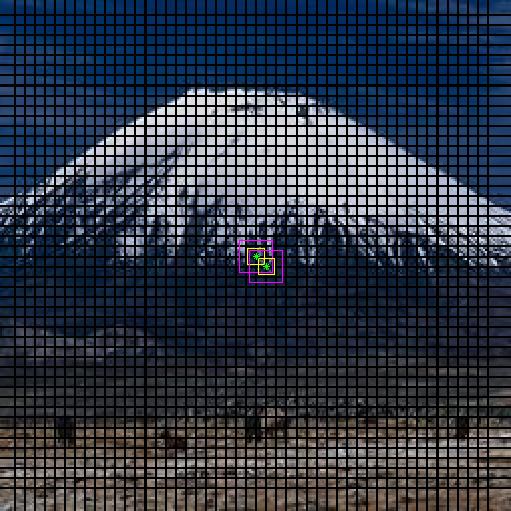
\includegraphics[scale = 0.65]{./images/LFflow/rect_crop.png}}
                \caption{Πλέγμα εικόνας με τις γειτονιές δύο κόμβων}
        \end{subfigure}
		
        \centering
        \begin{subfigure}[b]{0.2\textwidth}
                \centerline{
\includegraphics[scale = 0.35]{./images/LFflow/croppedLarge_crop.png}}
                \caption{}\label{subfig:pregauss1}
        \end{subfigure}%
		~
        \centering
        \begin{subfigure}[b]{0.2\textwidth}
                \centerline{
\includegraphics[scale = 0.45]{./images/LFflow/filteredLarge_crop.png}}
                \caption{}\label{subfig:gauss1}
        \end{subfigure}%
		~
        \centering
        \begin{subfigure}[b]{0.2\textwidth}
                \centerline{
\includegraphics[scale = 0.45]{./images/LFflow/croppedSmall_crop.png}}
                \caption{}\label{subfig:pregauss2}
        \end{subfigure}%
		~
        \centering
        \begin{subfigure}[b]{0.2\textwidth}
                \centerline{
\includegraphics[scale = 0.55]{./images/LFflow/filteredSmall_crop.png}}
                \caption{}\label{subfig:gauss2}
        \end{subfigure}%
        \caption{Πλέγμα σε εικόνα και γειτονιές πριν και μετά την εφαρμογή της Γκαουσιανής συνάρτησης}
        \label{fig:mountain}
\end{figure}





% ===========================================================================================================================
% ===========================================================================================================================
%\subsection{Δημιουργία των Codebooks}
%\paragraph*{}
%Το επόμενο βήμα είναι η δημιουργία των codebooks, έτσι ώστε οι εικόνες να αναπαρασταθούν μέσω του μοντέλου Bag of Words (BoW model). Το μοντέλο BoW αντιμετωπίζει τις εικόνες όπως θα αντιμετώπιζε κανείς ένα έγγραφο κειμένου. Χωρίζει τα διάφορα χαρακτηριστικά της κάθε εικόνας σε εικονικές "λέξεις" και έτσι η κάθε εικόνα αναπαρίσταται από το πόσες και ποιες "λέξεις" περιέχει.
\paragraph*{Δημιουργία των Codebooks}
Για τη δημιουργία των Codebooks του κάθε περιγραφέα χρησιμοποιήθηκαν 1000 εικόνες διαφορετικές από το σύνολο που αναφέρθηκε στην προηγούμενη ενότητα. Συγκεκριμένα επιλέχθηκε τυχαία μία εικόνα από σχεδόν κάθε κλάση της \textbf{SUN2012}. Αυτό έγινε, προκειμένου οι εικονικές λέξεις που θα προκύψουν να είναι πιο αντικειμενικές και όχι "προσαρμοσμένες" στο σύνολο δεδομένων που θα ταξινομηθεί.

\paragraph*{}
Από τις 1000 εικόνες που επιλέχθηκαν, παράχθηκαν οι τοπικοί περιγραφείς τους. Στη συνέχεια, από αυτούς επιλέχθηκαν τυχαία 250.000, οι οποίοι τροφοδοτήθηκαν στον αλγόριθμο kmeans, με σκοπό την εύρεση ενός αριθμού κέντρων (π.χ. 512 ή 1024). Τα κέντρα αυτά έχουν τόσες διαστάσεις όσες και το μήκος των περιγραφέων και αποτελούν τις εικονικές λέξεις.

%Αναλυτικότερα, μετά την εξαγωγή των τοπικών περιγραφέων ενός ικανοποιητικού αριθμού εικόνων, επιλέγονται τυχαία κάποιοι από αυτούς για να παράξουν το codebook. Στη συνέχεια εφαρμόζεται ο αλγόριθμος kmeans στους τυχαία επιλεγμένους τοπικούς περιγραφείς, με σκοπό την εύρεση ενός αριθμού κέντρων (π.χ. 512 ή 1024). Τα κέντρα αυτά έχουν τόσες διαστάσεις όσες και το μήκος των περιγραφέων και αποτελούν τις εικονικές λέξεις.
%\paragraph*{}
%Προκειμένου να υπάρχει αντικειμενικότητα στα κέντρα που θα παράξει ο kmeans, για τη διαδικασία αυτή δε χρησιμοποιούνται οι 1921 εικόνες που αναφέρθηκαν στην προηγούμενη παράγραφο. Αντ' αυτού επιλέχθηκε τυχαία μία εικόνα από τις χίλιες πολυπληθέστερες κλάσεις της \textbf{SUN2012}. Αφού προσαρμόστηκε το μέγεθος όλων των εικόνων που επιλέχθηκαν, στη συνέχεια παράχθηκαν οι τοπικοί περιγραφείς τους. Από αυτούς, χρησιμοποιήθηκαν τυχαία 250.000, οι οποίοι τροφοδότησαν τον kmeans για την εύρεση των κέντρων.

% ===========================================================================================================================
% ===========================================================================================================================
\paragraph*{Δημιουργία των Feature Vectors}
Στη συνέχεια, προκειμένου να αναπαρασταθεί η κάθε εικόνα (πλέον από το σύνολο των 1921 εικόνων που επιλέχθηκαν για ταξινόμηση) με βάση τα Codebooks που δημιουργήθηκαν, υπολογίζεται η \textit{ευκλείδεια} απόσταση του κάθε τοπικού περιγραφέα από τα κέντρα που παράχθηκαν από τον kmeans και ο κάθε περιγραφέας αντιστοιχίζεται στο κοντινότερό του κέντρο. Τελικά τα feature vectors έχουν τόσα στοιχεία όσα και τα κέντρα που πάραξε κάθε φορά ο kmeans.

%Μετά τη δημιουργία των Codebooks, η κάθε εικόνα πρέπει να αναπαρασταθεί σύμφωνα με τις εικονικές λέξεις που έχουν προκύψει. Έτσι, για κάθε εικόνα γίνεται μία ταξινόμηση των τοπικών περιγραφέων, με βάση την απόσταση του καθενός από τα κέντρα που έχουν προκύψει. Τελικά η αναπαράσταση της κάθε εικόνας είναι το ιστόγραμμα των εικονικών λέξεων τις οποίες περιέχει. Στην ουσία, αυτό που χαρακτηρίζει την εικόνα είναι ένα διάνυσμα (feature vector) με μήκος όσα και τα κέντρα/εικονικές λέξεις. Το κάθε στοιχείο δίνει τον αριθμό των τοπικών περιγραφέων της εικόνας, οι οποίοι ταξινομήθηκαν στο αντίστοιχο κέντρο.

% ===========================================================================================================================
% ===========================================================================================================================
\subsection{Ταξινόμηση των εικόνων}
\paragraph*{}
Τέλος, η ταξινόμηση των εικόνων γίνεται με τον ταξινομητή SVM (Support Vector Machine) με χρήση του λογισμικού LIBSVM \cite{libsvm}. Πιο συγκεκριμένα, για κάθε κλάση εκτελείται δυαδική ταξινόμηση (Binary Classification). Αυτό σημαίνει, πως σε κάθε ταξινόμηση, η απόφαση του ταξινομητή έχει να κάνει με το αν μια εικόνα ανήκει ή όχι σε μία συγκεκριμένη κλάση, και δεν έχει να κάνει με την κλάση στην οποία ανήκει η εικόνα. Για την ακρίβεια, το αποτέλεσμα που δίνει ο ταξινομητής για την κάθε εικόνα, είναι η πιθανότητα αυτή να ανήκει στην προς εξέταση κλάση. Με αυτό τον τρόπο εκτελούνται είκοσι ταξινομήσεις, μία για την κάθε κλάση της SUN2012 που έχει επιλεγεί.

\paragraph*{}
Όσον αφορά στον SVM, επιλέγεται να χρησιμοποιεί τον RBF kernel (Radial Basis Function). Αυτό σημαίνει πως πρέπει να επιλεχθούν οι τιμές για δύο παραμέτρους, $C$ και $\gamma$. Οι προκαθορισμένες τιμές που χρησιμοποιεί ο LIBSVM είναι $C = 1$ και $\gamma = \frac{1}{Number Of Features}$. Αυτές είναι και οι τιμές που χρησιμοποιήθηκαν σε πρώτο στάδιο στα πειράματα. Στη συνέχεια έγινε επιλογή των βέλτιστων παραμέτρων $C$ και $\gamma$ για την κάθε κλάση. Αυτή η διαδικασία γίνεται με 3-fold Cross-Validation για κάθε κλάση. Ουσιαστικά εκτελούνται πολλές ταξινομήσεις για διάφορα $C$ και $\gamma$  από ένα μεγάλος εύρος τιμών και τελικά επιλέγονται για την κάθε κλάση τα $C$ και $\gamma$ που επιφέρουν το υψηλότερο Mean Average Precision.


% ===========================================================================================================================
% ===========================================================================================================================
\subsection{Αξιολόγηση των αποτελεσμάτων}
Στον κλάδο της ανάκτησης πληροφορίας (Information Retrieval) χρησιμοποιούνται κάποιες μετρικές αξιολόγησης της απόδοσης ενός ταξινομητή, οι οποίες αναλύονται σύντομα παρακάτω.

\paragraph*{Precision (Positive Predictive Value)}
Πρόκειται για το ποσοστό των δεδομένων που ταξινομήθηκαν σωστά σε σχέση με όλα τα δεδομένα που ταξινομήθηκαν στην εκάστοτε κλάση:

\begin{equation}
Precision = \dfrac{Number Of True Positives}{Number Of True Positives + Number Of False Positives}
\end{equation}
Το Precision λαμβάνει υπόψιν όλα τα δεδομένα του dataset. Για την περίπτωση που η ταξινόμηση υλοποιείται πιθανοτικά και τα δεδομένα μπορούν να καταταχθούν σύμφωνα με την πιθανότητά τους να ανήκουν σε κάποια κλάση, το Precision μπορεί να υπολογιστεί για κάποια συγκεκριμένη θέση της κατάταξης (cut-off rank), λαμβάνοντας υπόψιν μόνο τα δεδομένα που είναι ψηλότερα στη λίστα.

\paragraph*{Recall (Sensitivity)}
Είναι το ποσοστό των σωστά ταξινομημένων δεδομένων σε μια κλάση σε σχέση με το σύνολο των δεδομένων που ανήκουν σε αυτή:
\begin{equation}
Recall = \dfrac{Number Of True Positives}{Number Of True Positives + Number Of False Negatives}
\end{equation}

\paragraph*{Average Precision}
Οι μετρικές Precision και Recall βασίζονται στο σύνολο των δεδομένων που έχουν ταξινομηθεί. Όταν όμως ένας ταξινομητής κατατάσσει τα δεδομένα σύμφωνα με την πιθανότητα του καθενός να ανήκει σε κάποια κλάση, θα πρέπει να ληφθεί και αυτό το δεδομένο υπόψιν στην αξιολόγηση. Κατατάσσοντας τα δεδομένα σύμφωνα με την πιθανότητα που επιστρέφει ο ταξινομητής και υπολογίζοντας και τις δύο μετρικές σε κάθε θέση της κατάταξης, είναι δυνατό να εκφραστεί το Precision ως συνάρτηση του Recall και να σχεδιαστεί η καμπύλη $P(r)$. Το εμβαδόν κάτω από την καμπύλη είναι η τιμή του Average Precision. Εναλλακτικά μπορεί να υπολογιστεί από τον παρακάτω τύπο:
\begin{equation}
Average Precision = \dfrac{\sum_{k = 1}^{n}(P(k) \times rel(k))}{Number Of True Positives + Number Of False Negatives},
\end{equation}
όπου $k$ είναι η θέση στην κατάταξη των δεδομένων, $n$ ο αριθμός των δεδομένων, $P(k)$ το Precision στη θέση $k$ της κατάταξης και $rel(k)$ μια συνάρτηση, η οποία παίρνει την τιμή 1 αν το δεδομένο της θέσης $k$ ανήκει στην κλάση και την τιμή 0 αν δεν ανήκει.

\paragraph*{Mean Average Precision}
Αν έχουν διεξαχθεί $N$ ταξινομήσεις, τότε το Mean Average Precision είναι ο μέσος όρος των Average Precisions της κάθε ταξινόμησης:
\begin{equation}
Mean Average Precision = \dfrac{\sum_{n = 1}^{N}Average Precision(n)}{N}
\end{equation}

% =========================================================================================================================================
% =========================================================================================================================================

\section{Αποτελέσματα}
\subsection{Προτεινόμενος Περιγραφέας}
\paragraph*{}
Παρακάτω παρατίθενται τα αποτελέσματα των πειραμάτων που εκτελέστηκαν με τις προκαθορισμένες τιμές $C$ και $\gamma$, καθώς και μετά την επιλογή των βέλτιστων. Έγιναν δοκιμές για διαφορετικούς αριθμούς κέντρων για τον kmeans (256, 512 \& 1024), δηλαδή για διαφορετικά μήκη των Feature Vectors, για διαφορετικό αριθμό folds για το cross-validation (3, 10 \& 50) και για διαφορετικό αριθμό επιπέδων κβάντισης των γωνιών $\theta_1$ και $\theta_2$ (9 \& 10).

\paragraph*{}
Στους Πίνακες \ref{tab:default1} - \ref{tab:MAP2} φαίνεται το Mean Average Precision (MAP) για την κάθε κλάση, καθώς και η prior probablity της κάθε κλάσης. Συγκεκριμένα, οι Πίνακες \ref{tab:default1} - \ref{tab:default2}, έχουν τις τιμές των Mean Average Precisions για τις προκαθορισμένες τιμές $C = 1$ και $\gamma = \frac{1}{1921} = 0.000521$, ενώ οι Πίνακες \ref{tab:MAP1} - \ref{tab:MAP2} έχουν τις αντίστοιχες τιμές για τα βέλτιστα $(C, \gamma)$ που επιλέχθηκαν για κάθε κλάση. Στον Πίνακα \ref{tab:finalMAPs} δίνεται το συνολικό Mean Average Precision της κάθε ταξινόμησης (μέσος όρος των Mean Average Precisions της κάθε κλάσης).

% =======================================================================================================================================
% ====================== DEFAULT C, GAMMA ===============================================================================================
% =======================================================================================================================================

\begin{table}[!b]
\captionsetup{font={small}}
\caption[MAP κλάσεων με προκαθ. $(C, \gamma), Folds = 3$ \& $\abs{\theta_1} = \abs{\theta_2} = 9$]{MAP κλάσεων με προκαθορισμένα $(C, \gamma), Folds = 3$ \& $\abs{\theta_1} = \abs{\theta_2} = 9$}\label{tab:default1}
\centerline{ 
\begin{tabular}{c|c||c||c||c}
\textbf{Class}  & $\boldsymbol{k = 256}$ & $\boldsymbol{k = 512}$ & $\boldsymbol{k = 1024}$ & \textbf{Prior} \\ \hline
Art Studio      &  0.063894  &  0.081614  &  0.062726  &  0.041124 \\
Bathroom        &  0.127658  &  0.172253  &  0.176499  &  0.052057 \\
Beach           &  0.171324  &  0.186015  &  0.196122  &  0.050495 \\
Bedroom         &  0.184648  &  0.207515  &  0.220907  &  0.052056 \\
Building Facade &  0.129723  &  0.092083  &  0.102008  &  0.052057 \\
Coast           &  0.092556  &  0.123573  &  0.120666  &  0.049453 \\
Conference Room &  0.058287  &  0.0752    &  0.090511  &  0.04581  \\
Corridor        &  0.097436  &  0.160207  &  0.172728  &  0.049974 \\
Dining Room     &  0.136785  &  0.152057  &  0.165016  &  0.052057 \\
Game Room       &  0.102144  &  0.104751  &  0.117927  &  0.052056 \\
Highway         &  0.365122  &  0.436296  &  0.56936  &  0.052057 \\
Home Office     &  0.097321  &  0.095466  &  0.085475  &  0.042686 \\
Hotel Room      &  0.100107  &  0.084862  &  0.113705  &  0.052056 \\
Kitchen         &  0.091571  &  0.09959   &  0.148255  &  0.052057 \\
Living Room     &  0.10587   &  0.172773  &  0.118368  &  0.052057 \\
Mountain        &  0.122079  &  0.143805  &  0.167993  &  0.043727 \\
Mountain Snowy  &  0.120966  &  0.155292  &  0.188036  &  0.052056 \\
Skyscraper      &  0.108786  &  0.075136  &  0.074188  &  0.052057 \\
Street          &  0.227143  &  0.229103  &  0.313941  &  0.052057 \\
Waiting Room    &  0.124251  &  0.167801  &  0.164805  &  0.052056 \\
\end{tabular}
}
\end{table}


%\begin{table}
%\captionsetup{font={footnotesize}}
%\caption[MAP κλάσεων με προκαθ. $(C, \gamma)$ \& $Folds = 3, k = 512, \abs{\theta_1} = \abs{\theta_2} = 9$]{MAP κλάσεων με προκαθορισμένα $(C, \gamma)$ \& $Folds = 3, k = 512, \abs{\theta_1} = \abs{\theta_2} = 9$} 
%\centerline{ 
%\begin{tabular}{c||c||c}
%\textbf{Class}  & \textbf{MAP} & \textbf{Prior} \\ \hline
%Art Studio      & 0.081614 & 0.041124 \\
%Bathroom        & 0.172253 & 0.052057 \\
%Beach           & 0.186015  & 0.050495 \\
%Bedroom         & 0.207515 & 0.052056 \\
%Building Facade & 0.092083  & 0.052057 \\
%Coast           & 0.123573 & 0.049453 \\
%Conference Room & 0.0752 & 0.04581  \\
%Corridor        & 0.160207 & 0.049974 \\
%Dining Room     & 0.152057 & 0.052057 \\
%Game Room       & 0.104751 & 0.052056 \\
%Highway         & 0.436296 & 0.052057 \\
%Home Office     & 0.095466 & 0.042686 \\
%Hotel Room      & 0.084862 & 0.052056 \\
%Kitchen         & 0.09959  & 0.052057 \\
%Living Room     & 0.172773  & 0.052057 \\
%Mountain        & 0.143805 & 0.043727 \\
%Mountain Snowy  & 0.155292 & 0.052056 \\
%Skyscraper      & 0.075136 & 0.052057 \\
%Street          & 0.229103 & 0.052057 \\
%Waiting Room    & 0.167801 & 0.052056 \\
%\end{tabular}
%}
%\end{table}


%\begin{table}
%\captionsetup{font={footnotesize}}
%\caption[MAP κλάσεων με προκαθ. $(C, \gamma)$ \& $Folds = 3, k = 1024, \abs{\theta_1} = \abs{\theta_2} = 9$]{MAP κλάσεων με προκαθορισμένα $(C, \gamma)$ \& $Folds = 3, k = 1024, \abs{\theta_1} = \abs{\theta_2} = 9$} 
%\centerline{ 
%\begin{tabular}{c||c||c}
%\textbf{Class}  & \textbf{MAP} & \textbf{Prior} \\ \hline
%Art Studio      & 0.062726 & 0.041124 \\
%Bathroom        & 0.176499 & 0.052057 \\
%Beach           & 0.196122  & 0.050495 \\
%Bedroom         & 0.220907 & 0.052056 \\
%Building Facade & 0.102008  & 0.052057 \\
%Coast           & 0.120666 & 0.049453 \\
%Conference Room & 0.090511 & 0.04581  \\
%Corridor        & 0.172728 & 0.049974 \\
%Dining Room     & 0.165016 & 0.052057 \\
%Game Room       & 0.117927 & 0.052056 \\
%Highway         & 0.56936 & 0.052057 \\
%Home Office     & 0.085475 & 0.042686 \\
%Hotel Room      & 0.113705 & 0.052056 \\
%Kitchen         & 0.148255  & 0.052057 \\
%Living Room     & 0.118368  & 0.052057 \\
%Mountain        & 0.167993 & 0.043727 \\
%Mountain Snowy  & 0.188036 & 0.052056 \\
%Skyscraper      & 0.074188 & 0.052057 \\
%Street          & 0.313941 & 0.052057 \\
%Waiting Room    & 0.164805 & 0.052056 \\
%\end{tabular}
%}
%\end{table}



\begin{table}
\captionsetup{font={small}}
\caption[MAP κλάσεων με προκαθ. $(C, \gamma), Folds = 10$ \& $\abs{\theta_1} = \abs{\theta_2} = 9$]{MAP κλάσεων με προκαθορισμένα $(C, \gamma)$ \& $Folds = 10, \abs{\theta_1} = \abs{\theta_2} = 9$} 
\centerline{ 
\begin{tabular}{c|c||c||c||c}
\textbf{Class}  & $\boldsymbol{k = 256}$ & $\boldsymbol{k = 512}$ & $\boldsymbol{k = 1024}$ & \textbf{Prior} \\ \hline
Art Studio      &  0.075893  &  0.095064  &  0.082852  &  0.041124 \\
Bathroom        &  0.146942  &  0.205189  &  0.209388  &  0.052056 \\
Beach           &  0.222928  &  0.203886  &  0.26532   &  0.050494 \\
Bedroom         &  0.205259  &  0.255747  &  0.238645  &  0.052056 \\
Building Facade &  0.146719  &  0.111306  &  0.134056  &  0.052056 \\
Coast           &  0.127882  &  0.131593  &  0.154347  &  0.049452 \\
Conference Room &  0.080869  &  0.088459  &  0.08354   &  0.045812  \\
Corridor        &  0.119455  &  0.157869  &  0.24166   &  0.049973 \\
Dining Room     &  0.142322  &  0.181586  &  0.213156  &  0.052056 \\
Game Room       &  0.109764  &  0.106966  &  0.140139  &  0.052056 \\
Highway         &  0.415427  &  0.450306  &  0.628165  &  0.052056 \\
Home Office     &  0.10405   &  0.116504  &  0.126226  &  0.042687 \\
Hotel Room      &  0.098973  &  0.109223  &  0.150421  &  0.052056 \\
Kitchen         &  0.128514  &  0.122073  &  0.17325   &  0.052056 \\
Living Room     &  0.164139  &  0.186187  &  0.209028  &  0.052056 \\
Mountain        &  0.145021  &  0.156785  &  0.224321  &  0.043726 \\
Mountain Snowy  &  0.168448  &  0.12648   &  0.242898  &  0.052056 \\
Skyscraper      &  0.135744  &  0.100235  &  0.130347  &  0.052056 \\
Street          &  0.247276  &  0.275991  &  0.364562  &  0.052056 \\
Waiting Room    &  0.158255  &  0.20499   &  0.193534  &  0.052056 \\
\end{tabular}
}
\end{table}



%\begin{table}
%\captionsetup{font={footnotesize}}
%\caption[MAP κλάσεων με προκαθ. $(C, \gamma)$ \& $Folds = 10, k = 512, \abs{\theta_1} = \abs{\theta_2} = 9$]{MAP κλάσεων με προκαθορισμένα $(C, \gamma)$ \& $Folds = 10, k = 512, \abs{\theta_1} = \abs{\theta_2} = 9$} 
%\centerline{ 
%\begin{tabular}{c||c||c}
%\textbf{Class}  & \textbf{MAP} & \textbf{Prior} \\ \hline
%Art Studio      & 0.095064 & 0.041124 \\
%Bathroom        & 0.205189 & 0.052056 \\
%Beach           & 0.203886  & 0.050494 \\
%Bedroom         & 0.255747 & 0.052056 \\
%Building Facade & 0.111306  & 0.052056 \\
%Coast           & 0.131593 & 0.049452 \\
%Conference Room & 0.088459 & 0.045812  \\
%Corridor        & 0.157869 & 0.049973 \\
%Dining Room     & 0.181586 & 0.052056 \\
%Game Room       & 0.106966 & 0.052056 \\
%Highway         & 0.450306 & 0.052056 \\
%Home Office     & 0.116504 & 0.042687 \\
%Hotel Room      & 0.109223 & 0.052056 \\
%Kitchen         & 0.122073  & 0.052056 \\
%Living Room     & 0.186187  & 0.052056 \\
%Mountain        & 0.156785 & 0.043726 \\
%Mountain Snowy  & 0.12648 & 0.052056 \\
%Skyscraper      & 0.100235 & 0.052056 \\
%Street          & 0.275991 & 0.052056 \\
%Waiting Room    & 0.20499 & 0.052056 \\
%\end{tabular}
%}
%\end{table}


%\begin{table}
%\captionsetup{font={footnotesize}}
%\caption[MAP κλάσεων με προκαθ. $(C, \gamma)$ \& $Folds = 10, k = 1024, \abs{\theta_1} = \abs{\theta_2} = 9$]{MAP κλάσεων με προκαθορισμένα $(C, \gamma)$ \& $Folds = 10, k = 1024, \abs{\theta_1} = \abs{\theta_2} = 9$} 
%\centerline{ 
%\begin{tabular}{c||c||c}
%\textbf{Class}  & \textbf{MAP} & \textbf{Prior} \\ \hline
%Art Studio      & 0.082852 & 0.041124 \\
%Bathroom        & 0.209388 & 0.052056 \\
%Beach           & 0.26532  & 0.050494 \\
%Bedroom         & 0.238645 & 0.052056 \\
%Building Facade & 0.134056  & 0.052056 \\
%Coast           & 0.154347 & 0.049452 \\
%Conference Room & 0.08354 & 0.045812  \\
%Corridor        & 0.24166 & 0.049973 \\
%Dining Room     & 0.213156 & 0.052056 \\
%Game Room       & 0.140139 & 0.052056 \\
%Highway         & 0.628165 & 0.052056 \\
%Home Office     & 0.126226 & 0.042687 \\
%Hotel Room      & 0.150421 & 0.052056 \\
%Kitchen         & 0.17325  & 0.052056 \\
%Living Room     & 0.209028  & 0.052056 \\
%Mountain        & 0.224321 & 0.043726 \\
%Mountain Snowy  & 0.242898 & 0.052056 \\
%Skyscraper      & 0.130347 & 0.052056 \\
%Street          & 0.364562 & 0.052056 \\
%Waiting Room    & 0.193534 & 0.052056 \\
%\end{tabular}
%}
%\end{table}



\begin{table}
\captionsetup{font={small}}
\caption[MAP κλάσεων με προκαθ. $(C, \gamma)$ \& $Folds = 50, \abs{\theta_1} = \abs{\theta_2} = 9$]{MAP κλάσεων με προκαθορισμένα $(C, \gamma)$ \& $Folds = 50, \abs{\theta_1} = \abs{\theta_2} = 9$} 
\centerline{ 
\begin{tabular}{c|c||c||c||c}
\textbf{Class}  & $\boldsymbol{k = 256}$ & $\boldsymbol{k = 512}$ & $\boldsymbol{k = 1024}$ & \textbf{Prior} \\ \hline
Art Studio      &  0.130312  &  0.18446   &  0.121163  &  0.041012 \\
Bathroom        &  0.266897  &  0.310006  &  0.286251  &  0.052065 \\
Beach           &  0.354134  &  0.327172  &  0.376761  &  0.050486 \\
Bedroom         &  0.284592  &  0.403264  &  0.389215  &  0.052065 \\
Building Facade &  0.203416  &  0.174679  &  0.214375  &  0.052065 \\
Coast           &  0.234959  &  0.250111  &  0.253457  &  0.049433 \\
Conference Room &  0.122138  &  0.150524  &  0.168396  &  0.045911  \\
Corridor        &  0.20066   &  0.291181  &  0.361927  &  0.050013 \\
Dining Room     &  0.296275  &  0.286858  &  0.333027  &  0.052065 \\
Game Room       &  0.20529   &  0.207475  &  0.258443  &  0.052065 \\
Highway         &  0.569267  &  0.56918   &  0.660474  &  0.052065 \\
Home Office     &  0.175708  &  0.244824  &  0.219133  &  0.042659 \\
Hotel Room      &  0.204079  &  0.211529  &  0.228224  &  0.052065 \\
Kitchen         &  0.202199  &  0.207997  &  0.291128  &  0.052065 \\
Living Room     &  0.240273  &  0.307667  &  0.317422  &  0.052065 \\
Mountain        &  0.270273  &  0.254283  &  0.303503  &  0.043644 \\
Mountain Snowy  &  0.252137  &  0.265486  &  0.326909  &  0.052065 \\
Skyscraper      &  0.220027  &  0.156197  &  0.214107  &  0.052065 \\
Street          &  0.408652  &  0.41957   &  0.483664  &  0.052065 \\
Waiting Room    &  0.274978  &  0.279101  &  0.341361  &  0.052065 \\
\end{tabular}
}
\end{table}



%\begin{table}
%\captionsetup{font={footnotesize}}
%\caption[MAP κλάσεων με προκαθ. $(C, \gamma)$ \& $Folds = 50, k = 512, \abs{\theta_1} = \abs{\theta_2} = 9$]{MAP κλάσεων με προκαθορισμένα $(C, \gamma)$ \& $Folds = 50, k = 512, \abs{\theta_1} = \abs{\theta_2} = 9$} 
%\centerline{ 
%\begin{tabular}{c||c||c}
%\textbf{Class}  & \textbf{MAP} & \textbf{Prior} \\ \hline
%Art Studio      & 0.18446 & 0.041012 \\
%Bathroom        & 0.310006 & 0.052065 \\
%Beach           & 0.327172  & 0.050486 \\
%Bedroom         & 0.403264 & 0.052065 \\
%Building Facade & 0.174679  & 0.052065 \\
%Coast           & 0.250111 & 0.049433 \\
%Conference Room & 0.150524 & 0.045911  \\
%Corridor        & 0.291181 & 0.050013 \\
%Dining Room     & 0.286858 & 0.052065 \\
%Game Room       & 0.207475 & 0.052065 \\
%Highway         & 0.56918 & 0.052065 \\
%Home Office     & 0.244824 & 0.042659 \\
%Hotel Room      & 0.211529 & 0.052065 \\
%Kitchen         & 0.207997  & 0.052065 \\
%Living Room     & 0.307667  & 0.052065 \\
%Mountain        & 0.254283 & 0.043644 \\
%Mountain Snowy  & 0.265486 & 0.052065 \\
%Skyscraper      & 0.156197 & 0.052065 \\
%Street          & 0.41957 & 0.052065 \\
%Waiting Room    & 0.279101 & 0.052065 \\
%\end{tabular}
%}
%\end{table}

%\begin{table}
%\captionsetup{font={footnotesize}}
%\caption[MAP κλάσεων με προκαθ. $(C, \gamma)$ \& $Folds = 50, k = 1024, \abs{\theta_1} = \abs{\theta_2} = 9$]{MAP κλάσεων με προκαθορισμένα $(C, \gamma)$ \& $Folds = 50, k = 1024, \abs{\theta_1} = \abs{\theta_2} = 9$} 
%\centerline{ 
%\begin{tabular}{c||c||c}
%\textbf{Class}  & \textbf{MAP} & \textbf{Prior} \\ \hline
%Art Studio      & 0.121163 & 0.041012 \\
%Bathroom        & 0.286251 & 0.052065 \\
%Beach           & 0.376761  & 0.050486 \\
%Bedroom         & 0.389215 & 0.052065 \\
%Building Facade & 0.214375  & 0.052065 \\
%Coast           & 0.253457 & 0.049433 \\
%Conference Room & 0.168396 & 0.045911  \\
%Corridor        & 0.361927 & 0.050013 \\
%Dining Room     & 0.333027 & 0.052065 \\
%Game Room       & 0.258443 & 0.052065 \\
%Highway         & 0.660474 & 0.052065 \\
%Home Office     & 0.219133 & 0.042659 \\
%Hotel Room      & 0.228224 & 0.052065 \\
%Kitchen         & 0.291128  & 0.052065 \\
%Living Room     & 0.317422  & 0.052065 \\
%Mountain        & 0.303503 & 0.043644 \\
%Mountain Snowy  & 0.326909 & 0.052065 \\
%Skyscraper      & 0.214107 & 0.052065 \\
%Street          & 0.483664 & 0.052065 \\
%Waiting Room    & 0.341361 & 0.052065 \\
%\end{tabular}
%}
%\end{table}



\begin{table}
\captionsetup{font={small}}
\caption[MAP κλάσεων με προκαθ. $(C, \gamma), Folds = 3$ \& $\abs{\theta_1} = \abs{\theta_2} = 10$]{MAP κλάσεων με προκαθορισμένα $(C, \gamma), Folds = 3$ \& $\abs{\theta_1} = \abs{\theta_2} = 10$} 
\centerline{ 
\begin{tabular}{c|c||c||c||c}
\textbf{Class}  & $\boldsymbol{k = 256}$ & $\boldsymbol{k = 512}$ & $\boldsymbol{k = 1024}$ & \textbf{Prior} \\ \hline
Art Studio      &  0.079997  &  0.080263  &  0.073313  &  0.041124 \\
Bathroom        &  0.137565  &  0.139438  &  0.157811  &  0.052057 \\
Beach           &  0.248308  &  0.15636   &  0.199223  &  0.050495 \\
Bedroom         &  0.214903  &  0.21657   &  0.261672  &  0.052056 \\
Building Facade &  0.112144  &  0.116477  &  0.161065  &  0.052057 \\
Coast           &  0.116706  &  0.12779   &  0.119791  &  0.049453 \\
Conference Room &  0.078096  &  0.077753  &  0.086691  &  0.04581  \\
Corridor        &  0.085352  &  0.119937  &  0.175487  &  0.049974 \\
Dining Room     &  0.161409  &  0.149748  &  0.24039   &  0.052057 \\
Game Room       &  0.099058  &  0.125394  &  0.089614  &  0.052056 \\
Highway         &  0.388948  &  0.376431  &  0.542788  &  0.052057 \\
Home Office     &  0.071432  &  0.117242  &  0.093314  &  0.042686 \\
Hotel Room      &  0.088796  &  0.118469  &  0.10698   &  0.052056 \\
Kitchen         &  0.146953  &  0.161449  &  0.176027  &  0.052057 \\
Living Room     &  0.076906  &  0.117852  &  0.153996  &  0.052057 \\
Mountain        &  0.070386  &  0.081114  &  0.120512  &  0.043727 \\
Mountain Snowy  &  0.116827  &  0.170581  &  0.152396  &  0.052056 \\
Skyscraper      &  0.082739  &  0.07459   &  0.105786  &  0.052057 \\
Street          &  0.209066  &  0.220444  &  0.296925  &  0.052057 \\
Waiting Room    &  0.08409   &  0.079781  &  0.123116  &  0.052056 \\
\end{tabular}
}
\end{table}

%\begin{table}
%\captionsetup{font={footnotesize}}
%\caption[MAP κλάσεων με προκαθ. $(C, \gamma)$ \& $Folds = 3, k = 512, \abs{\theta_1} = \abs{\theta_2} = 10$]{MAP κλάσεων με προκαθορισμένα $(C, \gamma)$ \& $Folds = 3, k = 512, \abs{\theta_1} = \abs{\theta_2} = 10$} 
%\centerline{ 
%\begin{tabular}{c||c||c}
%\textbf{Class}  & \textbf{MAP} & \textbf{Prior} \\ \hline
%Art Studio      & 0.080263 & 0.041124 \\
%Bathroom        & 0.139438 & 0.052057 \\
%Beach           & 0.15636  & 0.050495 \\
%Bedroom         & 0.21657 & 0.052056 \\
%Building Facade & 0.116477  & 0.052057 \\
%Coast           & 0.12779 & 0.049453 \\
%Conference Room & 0.077753 & 0.04581  \\
%Corridor        & 0.119937 & 0.049974 \\
%Dining Room     & 0.149748 & 0.052057 \\
%Game Room       & 0.125394 & 0.052056 \\
%Highway         & 0.376431 & 0.052057 \\
%Home Office     & 0.117242 & 0.042686 \\
%Hotel Room      & 0.118469 & 0.052056 \\
%Kitchen         & 0.161449  & 0.052057 \\
%Living Room     & 0.117852  & 0.052057 \\
%Mountain        & 0.081114 & 0.043727 \\
%Mountain Snowy  & 0.170581 & 0.052056 \\
%Skyscraper      & 0.07459 & 0.052057 \\
%Street          & 0.220444 & 0.052057 \\
%Waiting Room    & 0.079781 & 0.052056 \\
%\end{tabular}
%}
%\end{table}


%\begin{table}
%\captionsetup{font={footnotesize}}
%\caption[MAP κλάσεων με προκαθ. $(C, \gamma)$ \& $Folds = 3, k = 1024, \abs{\theta_1} = \abs{\theta_2} = 10$]{MAP κλάσεων με προκαθορισμένα $(C, \gamma)$ \& $Folds = 3, k = 1024, \abs{\theta_1} = \abs{\theta_2} = 10$} 
%\centerline{ 
%\begin{tabular}{c||c||c}
%\textbf{Class}  & \textbf{MAP} & \textbf{Prior} \\ \hline
%Art Studio      & 0.073313 & 0.041124 \\
%Bathroom        & 0.157811 & 0.052057 \\
%Beach           & 0.199223  & 0.050495 \\
%Bedroom         & 0.261672 & 0.052056 \\
%Building Facade & 0.161065  & 0.052057 \\
%Coast           & 0.119791 & 0.049453 \\
%Conference Room & 0.086691 & 0.04581  \\
%Corridor        & 0.175487 & 0.049974 \\
%Dining Room     & 0.24039 & 0.052057 \\
%Game Room       & 0.089614 & 0.052056 \\
%Highway         & 0.542788 & 0.052057 \\
%Home Office     & 0.093314 & 0.042686 \\
%Hotel Room      & 0.10698 & 0.052056 \\
%Kitchen         & 0.176027  & 0.052057 \\
%Living Room     & 0.153996  & 0.052057 \\
%Mountain        & 0.120512 & 0.043727 \\
%Mountain Snowy  & 0.152396 & 0.052056 \\
%Skyscraper      & 0.105786 & 0.052057 \\
%Street          & 0.296925 & 0.052057 \\
%Waiting Room    & 0.123116 & 0.052056 \\
%\end{tabular}
%}
%\end{table}


\begin{table}
\captionsetup{font={small}}
\caption[MAP κλάσεων με προκαθ. $(C, \gamma, Folds = 10$ \& $\abs{\theta_1} = \abs{\theta_2} = 10$]{MAP κλάσεων με προκαθορισμένα $(C, \gamma), Folds = 10$ \& $\abs{\theta_1} = \abs{\theta_2} = 10$} 
\centerline{ 
\begin{tabular}{c|c||c||c||c}
\textbf{Class}  & $\boldsymbol{k = 256}$ & $\boldsymbol{k = 512}$ & $\boldsymbol{k = 1024}$ & \textbf{Prior} \\ \hline
Art Studio      &  0.105937  &  0.098698  &  0.100495  &  0.041124 \\
Bathroom        &  0.190204  &  0.177112  &  0.156943  &  0.052056 \\
Beach           &  0.259469  &  0.158145  &  0.222484  &  0.050494 \\
Bedroom         &  0.231609  &  0.274107  &  0.303034  &  0.052056 \\
Building Facade &  0.13816   &  0.157389  &  0.183472  &  0.052056 \\
Coast           &  0.155485  &  0.173137  &  0.129701  &  0.049452 \\
Conference Room &  0.13393   &  0.103576  &  0.117282  &  0.045812  \\
Corridor        &  0.096897  &  0.143852  &  0.203655  &  0.049973 \\
Dining Room     &  0.205306  &  0.175017  &  0.2979    &  0.052056 \\
Game Room       &  0.139024  &  0.16479   &  0.134975  &  0.052056 \\
Highway         &  0.425514  &  0.529444  &  0.530649  &  0.052056 \\
Home Office     &  0.090303  &  0.133913  &  0.123546  &  0.042687 \\
Hotel Room      &  0.120336  &  0.129741  &  0.141975  &  0.052056 \\
Kitchen         &  0.196764  &  0.202736  &  0.200472  &  0.052056 \\
Living Room     &  0.116226  &  0.12239   &  0.193498  &  0.052056 \\
Mountain        &  0.131725  &  0.154989  &  0.144307  &  0.043726 \\
Mountain Snowy  &  0.183736  &  0.212613  &  0.177229  &  0.052056 \\
Skyscraper      &  0.104785  &  0.125049  &  0.11931   &  0.052056 \\
Street          &  0.292208  &  0.286966  &  0.327008  &  0.052056 \\
Waiting Room    &  0.138026  &  0.100611  &  0.163523  &  0.052056 \\
\end{tabular}
}
\end{table}


%\begin{table}
%\captionsetup{font={footnotesize}}
%\caption[MAP κλάσεων με προκαθ. $(C, \gamma)$ \& $Folds = 10, k = 512, \abs{\theta_1} = \abs{\theta_2} = 10$]{MAP κλάσεων με προκαθορισμένα $(C, \gamma)$ \& $Folds = 10, k = 512, \abs{\theta_1} = \abs{\theta_2} = 10$} 
%\centerline{ 
%\begin{tabular}{c||c||c}
%\textbf{Class}  & \textbf{MAP} & \textbf{Prior} \\ \hline
%Art Studio      & 0.098698 & 0.041124 \\
%Bathroom        & 0.177112 & 0.052056 \\
%Beach           & 0.158145  & 0.050494 \\
%Bedroom         & 0.274107 & 0.052056 \\
%Building Facade & 0.157389  & 0.052056 \\
%Coast           & 0.173137 & 0.049452 \\
%Conference Room & 0.103576 & 0.045812  \\
%Corridor        & 0.143852 & 0.049973 \\
%Dining Room     & 0.175017 & 0.052056 \\
%Game Room       & 0.16479 & 0.052056 \\
%Highway         & 0.529444 & 0.052056 \\
%Home Office     & 0.133913 & 0.042687 \\
%Hotel Room      & 0.129741 & 0.052056 \\
%Kitchen         & 0.202736  & 0.052056 \\
%Living Room     & 0.12239  & 0.052056 \\
%Mountain        & 0.154989 & 0.043726 \\
%Mountain Snowy  & 0.212613 & 0.052056 \\
%Skyscraper      & 0.125049 & 0.052056 \\
%Street          & 0.286966 & 0.052056 \\
%Waiting Room    & 0.100611 & 0.052056 \\
%\end{tabular}
%}
%\end{table}


%\begin{table}
%\captionsetup{font={footnotesize}}
%\caption[MAP κλάσεων με προκαθ. $(C, \gamma)$ \& $Folds = 10, k = 1024, \abs{\theta_1} = \abs{\theta_2} = 10$]{MAP κλάσεων με προκαθορισμένα $(C, \gamma)$ \& $Folds = 10, k = 1024, \abs{\theta_1} = \abs{\theta_2} = 10$} 
%\centerline{ 
%\begin{tabular}{c||c||c}
%\textbf{Class}  & \textbf{MAP} & \textbf{Prior} \\ \hline
%Art Studio      & 0.100495 & 0.041124 \\
%Bathroom        & 0.156943 & 0.052056 \\
%Beach           & 0.222484  & 0.050494 \\
%Bedroom         & 0.303034 & 0.052056 \\
%Building Facade & 0.183472  & 0.052056 \\
%Coast           & 0.129701 & 0.049452 \\
%Conference Room & 0.117282 & 0.045812  \\
%Corridor        & 0.203655 & 0.049973 \\
%Dining Room     & 0.2979 & 0.052056 \\
%Game Room       & 0.134975 & 0.052056 \\
%Highway         & 0.530649 & 0.052056 \\
%Home Office     & 0.123546 & 0.042687 \\
%Hotel Room      & 0.141975 & 0.052056 \\
%Kitchen         & 0.200472  & 0.052056 \\
%Living Room     & 0.193498  & 0.052056 \\
%Mountain        & 0.144307 & 0.043726 \\
%Mountain Snowy  & 0.177229 & 0.052056 \\
%Skyscraper      & 0.11931 & 0.052056 \\
%Street          & 0.327008 & 0.052056 \\
%Waiting Room    & 0.163523 & 0.052056 \\
%\end{tabular}
%}
%\end{table}


\begin{table}[!t]
\captionsetup{font={small}}
\caption[MAP κλάσεων με προκαθ. $(C, \gamma), Folds = 50$ \& $\abs{\theta_1} = \abs{\theta_2} = 10$]{MAP κλάσεων με προκαθορισμένα $(C, \gamma), Folds = 50$ \& $\abs{\theta_1} = \abs{\theta_2} = 10$} \label{tab:default2}
\centerline{ 
\begin{tabular}{c|c||c||c||c}
\textbf{Class}  & $\boldsymbol{k = 256}$ & $\boldsymbol{k = 512}$ & $\boldsymbol{k = 1024}$ & \textbf{Prior} \\ \hline
Art Studio      &  0.205115  &  0.173588  &  0.188372  &  0.041012 \\
Bathroom        &  0.272554  &  0.240376  &  0.279552  &  0.052065 \\
Beach           &  0.391903  &  0.29667   &  0.334888  &  0.050486 \\
Bedroom         &  0.336184  &  0.404155  &  0.434131  &  0.052065 \\
Building Facade &  0.233229  &  0.260713  &  0.248968  &  0.052065 \\
Coast           &  0.180767  &  0.304528  &  0.229332  &  0.049433 \\
Conference Room &  0.197017  &  0.180601  &  0.203306  &  0.045911 \\
Corridor        &  0.185167  &  0.216838  &  0.26654   &  0.050013 \\
Dining Room     &  0.32361   &  0.320754  &  0.37075   &  0.052065 \\
Game Room       &  0.22486   &  0.266379  &  0.231751  &  0.052065 \\
Highway         &  0.534109  &  0.604833  &  0.650643  &  0.052065 \\
Home Office     &  0.189517  &  0.239148  &  0.237753  &  0.042659 \\
Hotel Room      &  0.202306  &  0.19976   &  0.209218  &  0.052065 \\
Kitchen         &  0.300351  &  0.334994  &  0.325579  &  0.052065 \\
Living Room     &  0.193113  &  0.196667  &  0.291978  &  0.052065 \\
Mountain        &  0.20063   &  0.273075  &  0.277964  &  0.043644 \\
Mountain Snowy  &  0.232507  &  0.29957   &  0.333334  &  0.052065 \\
Skyscraper      &  0.217296  &  0.222932  &  0.194985  &  0.052065 \\
Street          &  0.428378  &  0.451346  &  0.48494   &  0.052065 \\
Waiting Room    &  0.226862  &  0.183279  &  0.277651  &  0.052065 \\
\end{tabular}
}
\end{table}
\newpage
\paragraph*{}
Τα παραπάνω αποτελέσματα, δείχνουν πως, ακόμα και σε πρωταρχικό στάδιο, ο προτεινόμενος περιγραφέας έχει καλή απόδοση. Το σημαντικότερο είναι πως, ακόμα και για τα χαμηλότερα MAPs που εμφανίζονται, δεν πέφτουν \textit{ποτέ} κάτω από την prior probability της κάθε κλάσης, που είναι το ποσοστό των εικόνων της εκάστοτε κλάσης σε σχέση με όλο το σύνολο των εικόνων.Αυτή θα ήταν η απόδοση που θα είχε ένας τυχαίος ταξινομητής. Επιπλέον, είναι εμφανές πως καθώς αυξάνεται ο αριθμός των folds, αυξάνεται και η απόδοση της ταξινόμησης. Επίσης η αύξηση των εικονικών λέξεων, σε γενικές γραμμές προκαλεί αύξηση του MAP της κάθε κλάσης, όμως η αύξηση/μείωση των παραμέτρων $\theta_1, \theta_2$ δεν εμφανίζει ξεκάθαρη αλλαγή, αλλά η κάθε κλάση επηρεάζεται διαφορετικά.


%\begin{table}
%\captionsetup{font={footnotesize}}
%\caption[MAP κλάσεων με προκαθ. $(C, \gamma)$ \& $Folds = 50, k = 512, \abs{\theta_1} = \abs{\theta_2} = 10$]{MAP κλάσεων με προκαθορισμένα $(C, \gamma)$ \& $Folds = 50, k = 512, \abs{\theta_1} = \abs{\theta_2} = 10$} 
%\centerline{ 
%\begin{tabular}{c||c||c}
%\textbf{Class}  & \textbf{MAP} & \textbf{Prior} \\ \hline
%Art Studio      & 0.173588 & 0.041012 \\
%Bathroom        & 0.240376 & 0.052065 \\
%Beach           & 0.29667  & 0.050486 \\
%Bedroom         & 0.404155 & 0.052065 \\
%Building Facade & 0.260713  & 0.052065 \\
%Coast           & 0.304528 & 0.049433 \\
%Conference Room & 0.180601 & 0.045911  \\
%Corridor        & 0.216838 & 0.050013 \\
%Dining Room     & 0.320754 & 0.052065 \\
%Game Room       & 0.266379 & 0.052065 \\
%Highway         & 0.604833 & 0.052065 \\
%Home Office     & 0.239148 & 0.042659 \\
%Hotel Room      & 0.19976 & 0.052065 \\
%Kitchen         & 0.334994  & 0.052065 \\
%Living Room     & 0.196667  & 0.052065 \\
%Mountain        & 0.273075 & 0.043644 \\
%Mountain Snowy  & 0.29957 & 0.052065 \\
%Skyscraper      & 0.222932 & 0.052065 \\
%Street          & 0.451346 & 0.052065 \\
%Waiting Room    & 0.183279 & 0.052065 \\
%\end{tabular}
%}
%\end{table}


%\begin{table}
%\captionsetup{font={footnotesize}}
%\caption[MAP κλάσεων με προκαθ. $(C, \gamma)$ \& $fFolds = 50, k = 1024, \abs{\theta_1} = \abs{\theta_2} = 10$]{MAP κλάσεων με προκαθορισμένα $(C, \gamma)$ \& $fFolds = 50, k = 1024, \abs{\theta_1} = \abs{\theta_2} = 10$} \label{tab:default2}
%\centerline{ 
%\begin{tabular}{c||c||c}
%\textbf{Class}  & \textbf{MAP} & \textbf{Prior} \\ \hline
%Art Studio      & 0.188372  & 0.041012 \\
%Bathroom        & 0.279552  & 0.052065 \\
%Beach           & 0.334888  & 0.050486 \\
%Bedroom         & 0.434131  & 0.052065 \\
%Building Facade & 0.248968  & 0.052065 \\
%Coast           & 0.229332  & 0.049433 \\
%Conference Room & 0.203306  & 0.045911  \\
%Corridor        & 0.26654   & 0.050013 \\
%Dining Room     & 0.37075   & 0.052065 \\
%Game Room       & 0.231751  & 0.052065 \\
%Highway         & 0.650643  & 0.052065 \\
%Home Office     & 0.237753  & 0.042659 \\
%Hotel Room      & 0.209218  & 0.052065 \\
%Kitchen         & 0.325579  & 0.052065 \\
%Living Room     & 0.291978  & 0.052065 \\
%Mountain        & 0.277964  & 0.043644 \\
%Mountain Snowy  & 0.333334  & 0.052065 \\
%Skyscraper      & 0.194985  & 0.052065 \\
%Street          & 0.48494   & 0.052065 \\
%Waiting Room    & 0.277651  & 0.052065 \\
%\end{tabular}
%}
%\end{table}
\clearpage


% =======================================================================================================================================
% ====================== PARAMETER SELECTION ============================================================================================
% =======================================================================================================================================


\begin{table}[!b]
\captionsetup{font={small}}
\caption{MAP κλάσεων με βέλτιστα $(C, \gamma), Folds = 3$ \& $\abs{\theta_1} = \abs{\theta_2} = 9$} \label{tab:MAP1}
\centerline{ 
\begin{tabular}{c|c||c||c||c}
\textbf{Class}  & $\boldsymbol{k = 256}$ & $\boldsymbol{k = 512}$ & $\boldsymbol{k = 1024}$ & \textbf{Prior} \\ \hline
Art Studio      &  1         &  1         &  1         &  0.041124 \\
Bathroom        &  0.362161  &  0.362161  &  0.362161  &  0.052057 \\
Beach           &  0.27993   &  0.230228  &  0.251213  &  0.050495 \\
Bedroom         &  0.150613  &  0.150177  &  0.150177  &  0.052056 \\
Building Facade &  0.09927   &  0.102852  &  0.090378  &  0.052057 \\
Coast           &  0.106875  &  0.107269  &  0.116797  &  0.049453 \\
Conference Room &  0.081763  &  0.087463  &  0.119224  &  0.04581  \\
Corridor        &  0.160346  &  0.186411  &  0.256522  &  0.049974 \\
Dining Room     &  0.192957  &  0.245521  &  0.239706  &  0.052057 \\
Game Room       &  0.167939  &  0.133436  &  0.142271  &  0.052056 \\
Highway         &  0.523908  &  0.52981   &  0.60895   &  0.052057 \\
Home Office     &  0.162221  &  0.142854  &  0.148534  &  0.042686 \\
Hotel Room      &  0.134094  &  0.123842  &  0.15608   &  0.052056 \\
Kitchen         &  0.10016   &  0.245099  &  0.114369  &  0.052057 \\
Living Room     &  0.18249   &  0.207072  &  0.205403  &  0.052057 \\
Mountain        &  0.143669  &  0.154363  &  0.135092  &  0.043727 \\
Mountain Snowy  &  0.169751  &  0.18275   &  0.213666  &  0.052056 \\
Skyscraper      &  0.131846  &  0.119361  &  0.131357  &  0.052057 \\
Street          &  0.432261  &  0.493008  &  0.482712  &  0.052057 \\
Waiting Room    &  0.174738  &  0.184992  &  0.181842  &  0.052056 \\
\end{tabular}
}
\end{table}


%\begin{table}
%\captionsetup{font={small}}
%\caption{MAP κλάσεων με βέλτιστα $(C, \gamma)$ \& $Folds = 3, k = 512, \abs{\theta_1} = \abs{\theta_2} = 9$}
%\centerline{ 
%\begin{tabular}{c||c||c}
%\textbf{Class}           & \textbf{MAP}      & \textbf{Prior}    \\ \hline
%Art Studio      & 1        & 0.041124 \\
%Bathroom        & 0.362161 & 0.052057 \\
%Beach           & 0.230228 & 0.050495 \\
%Bedroom         & 0.150177 & 0.052056 \\
%Building Facade & 0.102852 & 0.052057 \\
%Coast           & 0.107269 & 0.049453 \\
%Conference Room & 0.087463 & 0.04581  \\
%Corridor        & 0.186411 & 0.049974 \\
%Dining Room     & 0.245521 & 0.052057 \\
%Game Room       & 0.133436 & 0.052056 \\
%Highway         & 0.52981  & 0.052057 \\
%Home Office     & 0.142854 & 0.042686 \\
%Hotel Room      & 0.123842 & 0.052056 \\
%Kitchen         & 0.245099 & 0.052057 \\
%Living Room     & 0.207072 & 0.052057 \\
%Mountain        & 0.154363 & 0.043727 \\
%Mountain Snowy  & 0.18275  & 0.052056 \\
%Skyscraper      & 0.119361 & 0.052057 \\
%Street          & 0.493008 & 0.052057 \\
%Waiting Room    & 0.184992 & 0.052056 \\
%\end{tabular}
%}
%\end{table}


%\begin{table}
%\captionsetup{font={small}}
%\caption{MAP κλάσεων με βέλτιστα $(C, \gamma)$ \& $Folds = 3, k = 1024, \abs{\theta_1} = \abs{\theta_2} = 9$}
%\centerline{ 
%\begin{tabular}{c||c||c}
%\textbf{Class}           & \textbf{MAP}      & \textbf{Prior}    \\ \hline
%Art Studio      & 1        & 0.041124 \\
%Bathroom        & 0.362161 & 0.052057 \\
%Beach           & 0.251213 & 0.050495 \\
%Bedroom         & 0.150177 & 0.052056 \\
%Building Facade & 0.090378 & 0.052057 \\
%Coast           & 0.116797 & 0.049453 \\
%Conference Room & 0.119224 & 0.04581  \\
%Corridor        & 0.256522 & 0.049974 \\
%Dining Room     & 0.239706 & 0.052057 \\
%Game Room       & 0.142271 & 0.052056 \\
%Highway         & 0.60895  & 0.052057 \\
%Home Office     & 0.148534 & 0.042686 \\
%Hotel Room      & 0.15608  & 0.052056 \\
%Kitchen         & 0.114369 & 0.052057 \\
%Living Room     & 0.205403 & 0.052057 \\
%Mountain        & 0.135092 & 0.043727 \\
%Mountain Snowy  & 0.213666 & 0.052056 \\
%Skyscraper      & 0.131357 & 0.052057 \\
%Street          & 0.482712 & 0.052057 \\
%Waiting Room    & 0.181842 & 0.052056 \\
%\end{tabular}
%}
%\end{table}


\begin{table}
\captionsetup{font={small}}
\caption{MAP κλάσεων με βέλτιστα $(C, \gamma), Folds = 10$ \& $\abs{\theta_1} = \abs{\theta_2} = 9$}
\centerline{ 
\begin{tabular}{c|c||c||c||c}
\textbf{Class}  & $\boldsymbol{k = 256}$ & $\boldsymbol{k = 512}$ & $\boldsymbol{k = 1024}$ & \textbf{Prior} \\ \hline
Art Studio      &  1         &  1         &  1  &  0.041124 \\
Bathroom        &  0.381111  &  0.381111  &  0.381111  &  0.052056 \\
Beach           &  0.300283  &  0.307213  &  0.274325  &  0.050494 \\
Bedroom         &  0.159832  &  0.157614  &  0.157563  &  0.052056 \\
Building Facade &  0.116547  &  0.131857  &  0.14746   &  0.052056 \\
Coast           &  0.139279  &  0.12674   &  0.145841  &  0.049452 \\
Conference Room &  0.104225  &  0.121341  &  0.145573  &  0.045812 \\
Corridor        &  0.235302  &  0.245513  &  0.321208  &  0.049973 \\
Dining Room     &  0.274234  &  0.315362  &  0.32545   &  0.052056 \\
Game Room       &  0.208783  &  0.171839  &  0.157295  &  0.052056 \\
Highway         &  0.570014  &  0.553496  &  0.609362  &  0.052056 \\
Home Office     &  0.181871  &  0.177636  &  0.177327  &  0.042687 \\
Hotel Room      &  0.174673  &  0.184601  &  0.179643  &  0.052056 \\
Kitchen         &  0.173119  &  0.162082  &  0.138157  &  0.052056 \\
Living Room     &  0.217057  &  0.251561  &  0.279407  &  0.052056 \\
Mountain        &  0.183148  &  0.222426  &  0.209991  &  0.043726 \\
Mountain Snowy  &  0.207899  &  0.207675  &  0.258425  &  0.052056 \\
Skyscraper      &  0.130135  &  0.141833  &  0.119368  &  0.052056 \\
Street          &  0.502054  &  0.490369  &  0.49149   &  0.052056 \\
Waiting Room    &  0.21356   &  0.22363   &  0.197682  &  0.052056 \\
\end{tabular}
}
\end{table}

%
%\begin{table}
%\captionsetup{font={small}}
%\caption{MAP κλάσεων με βέλτιστα $(C, \gamma)$ \& $Folds = 10, k = 512, \abs{\theta_1} = \abs{\theta_2} = 9$}
%\centerline{ 
%\begin{tabular}{c||c||c}
%\textbf{Class}           & \textbf{MAP}      & \textbf{Prior}    \\ \hline
%Art Studio      & 1        & 0.041124 \\
%Bathroom        & 0.381111 & 0.052056 \\
%Beach           & 0.307213 & 0.050494 \\
%Bedroom         & 0.157614 & 0.052056 \\
%Building Facade & 0.131857 & 0.052056 \\
%Coast           & 0.12674  & 0.049452 \\
%Conference Room & 0.121341 & 0.045812 \\
%Corridor        & 0.245513 & 0.049973 \\
%Dining Room     & 0.315362 & 0.052056 \\
%Game Room       & 0.171839 & 0.052056 \\
%Highway         & 0.553496 & 0.052056 \\
%Home Office     & 0.177636 & 0.042687 \\
%Hotel Room      & 0.184601 & 0.052056 \\
%Kitchen         & 0.162082 & 0.052056 \\
%Living Room     & 0.251561 & 0.052056 \\
%Mountain        & 0.222426 & 0.043726 \\
%Mountain Snowy  & 0.207675 & 0.052056 \\
%Skyscraper      & 0.141833 & 0.052056 \\
%Street          & 0.490369 & 0.052056 \\
%Waiting Room    & 0.22363  & 0.052056 \\
%\end{tabular}
%}
%\end{table}


%\begin{table}
%\captionsetup{font={small}}
%\caption{MAP κλάσεων με βέλτιστα $(C, \gamma)$ \& $Folds = 10, k = 1024, \abs{\theta_1} = \abs{\theta_2} = 9$}
%\centerline{ 
%\begin{tabular}{c||c||c}
%\textbf{Class}           & \textbf{MAP}      & \textbf{Prior}    \\ \hline
%Art Studio      & 1        & 0.041124 \\
%Bathroom        & 0.381111 & 0.052056 \\
%Beach           & 0.274325 & 0.050494 \\
%Bedroom         & 0.157563 & 0.052056 \\
%Building Facade & 0.14746  & 0.052056 \\
%Coast           & 0.145841 & 0.049452 \\
%Conference Room & 0.145573 & 0.045812 \\
%Corridor        & 0.321208 & 0.049973 \\
%Dining Room     & 0.32545  & 0.052056 \\
%Game Room       & 0.157295 & 0.052056 \\
%Highway         & 0.609362 & 0.052056 \\
%Home Office     & 0.177327 & 0.042687 \\
%Hotel Room      & 0.179643 & 0.052056 \\
%Kitchen         & 0.138157 & 0.052056 \\
%Living Room     & 0.279407 & 0.052056 \\
%Mountain        & 0.209991 & 0.043726 \\
%Mountain Snowy  & 0.258425 & 0.052056 \\
%Skyscraper      & 0.119368 & 0.052056 \\
%Street          & 0.49149  & 0.052056 \\
%Waiting Room    & 0.197682 & 0.052056 \\
%\end{tabular}
%}
%\end{table}


\begin{table}
\captionsetup{font={small}}
\caption{MAP κλάσεων με βέλτιστα $(C, \gamma), Folds = 50$ \& $\abs{\theta_1} = \abs{\theta_2} = 9$}
\centerline{ 
\begin{tabular}{c|c||c||c||c}
\textbf{Class}  & $\boldsymbol{k = 256}$ & $\boldsymbol{k = 512}$ & $\boldsymbol{k = 1024}$ & \textbf{Prior} \\ \hline
Art Studio      &  1         &  1         &  1         &  0.041012 \\
Bathroom        &  0.486667  &  0.486667  &  0.486667  &  0.052065 \\
Beach           &  0.343087  &  0.346298  &  0.333929  &  0.050486 \\
Bedroom         &  0.210714  &  0.206508  &  0.208294  &  0.052065 \\
Building Facade &  0.193925  &  0.19873   &  0.253202  &  0.052065 \\
Coast           &  0.23059   &  0.218194  &  0.264315  &  0.049433 \\
Conference Room &  0.221471  &  0.191171  &  0.291819  &  0.045911 \\
Corridor        &  0.349622  &  0.355057  &  0.413583  &  0.050013 \\
Dining Room     &  0.367021  &  0.421257  &  0.393269  &  0.052065 \\
Game Room       &  0.314294  &  0.251372  &  0.265178  &  0.052065 \\
Highway         &  0.628059  &  0.671587  &  0.702652  &  0.052065 \\
Home Office     &  0.270956  &  0.315666  &  0.276838  &  0.042659 \\
Hotel Room      &  0.290959  &  0.28689   &  0.285223  &  0.052065 \\
Kitchen         &  0.27347   &  0.272288  &  0.240684  &  0.052065 \\
Living Room     &  0.32919   &  0.364879  &  0.365865  &  0.052065 \\
Mountain        &  0.280085  &  0.385309  &  0.295985  &  0.043644 \\
Mountain Snowy  &  0.286989  &  0.342161  &  0.362631  &  0.052065 \\
Skyscraper      &  0.20935   &  0.230934  &  0.239688  &  0.052065 \\
Street          &  0.574799  &  0.587352  &  0.592235  &  0.052065 \\
Waiting Room    &  0.294129  &  0.320549  &  0.331991  &  0.052065 \\
\end{tabular}
}
\end{table}


%\begin{table}
%\captionsetup{font={small}}
%\caption{MAP κλάσεων με βέλτιστα $(C, \gamma)$ \& $Folds = 50, k = 512, \abs{\theta_1} = \abs{\theta_2} = 9$}
%\centerline{ 
%\begin{tabular}{c||c||c}
%\textbf{Class}           & \textbf{MAP}      & \textbf{Prior}    \\ \hline
%Art Studio      & 1        & 0.041012 \\
%Bathroom        & 0.486667 & 0.052065 \\
%Beach           & 0.346298 & 0.050486 \\
%Bedroom         & 0.206508 & 0.052065 \\
%Building Facade & 0.19873  & 0.052065 \\
%Coast           & 0.218194 & 0.049433 \\
%Conference Room & 0.191171 & 0.045911 \\
%Corridor        & 0.355057 & 0.050013 \\
%Dining Room     & 0.421257 & 0.052065 \\
%Game Room       & 0.251372 & 0.052065 \\
%Highway         & 0.671587 & 0.052065 \\
%Home Office     & 0.315666 & 0.042659 \\
%Hotel Room      & 0.28689  & 0.052065 \\
%Kitchen         & 0.272288 & 0.052065 \\
%Living Room     & 0.364879 & 0.052065 \\
%Mountain        & 0.385309 & 0.043644 \\
%Mountain Snowy  & 0.342161 & 0.052065 \\
%Skyscraper      & 0.230934 & 0.052065 \\
%Street          & 0.587352 & 0.052065 \\
%Waiting Room    & 0.320549 & 0.052065 \\
%\end{tabular}
%}
%\end{table}


%\begin{table}
%\captionsetup{font={small}}
%\caption{MAP κλάσεων με βέλτιστα $(C, \gamma)$ \& $Folds = 50, k = 1024, \abs{\theta_1} = \abs{\theta_2} = 9$}
%\centerline{ 
%\begin{tabular}{c||c||c}
%\textbf{Class}           & \textbf{MAP}      & \textbf{Prior}    \\ \hline
%Art Studio      & 1        & 0.041012 \\
%Bathroom        & 0.486667 & 0.052065 \\
%Beach           & 0.333929 & 0.050486 \\
%Bedroom         & 0.208294 & 0.052065 \\
%Building Facade & 0.253202 & 0.052065 \\
%Coast           & 0.264315 & 0.049433 \\
%Conference Room & 0.291819 & 0.045911 \\
%Corridor        & 0.413583 & 0.050013 \\
%Dining Room     & 0.393269 & 0.052065 \\
%Game Room       & 0.265178 & 0.052065 \\
%Highway         & 0.702652 & 0.052065 \\
%Home Office     & 0.276838 & 0.042659 \\
%Hotel Room      & 0.285223 & 0.052065 \\
%Kitchen         & 0.240684 & 0.052065 \\
%Living Room     & 0.365865 & 0.052065 \\
%Mountain        & 0.295985 & 0.043644 \\
%Mountain Snowy  & 0.362631 & 0.052065 \\
%Skyscraper      & 0.239688 & 0.052065 \\
%Street          & 0.592235 & 0.052065 \\
%Waiting Room    & 0.331991 & 0.052065 \\
%\end{tabular}
%}
%\end{table}


\begin{table}
\captionsetup{font={small}}
\caption{MAP κλάσεων με βέλτιστα $(C, \gamma), Folds = 3$ \& $\abs{\theta_1} = \abs{\theta_2} = 10$}
\centerline{ 
\begin{tabular}{c|c||c||c||c}
\textbf{Class}  & $\boldsymbol{k = 256}$ & $\boldsymbol{k = 512}$ & $\boldsymbol{k = 1024}$ & \textbf{Prior} \\ \hline
Art Studio      &  1         &  1         &  1         &  0.041124 \\
Bathroom        &  0.362161  &  0.362161  &  0.362161  &  0.052057 \\
Beach           &  0.37884   &  0.24723   &  0.204693  &  0.050495 \\
Bedroom         &  0.280157  &  0.268146  &  0.150613  &  0.052056 \\
Building Facade &  0.191962  &  0.145636  &  0.181169  &  0.052057 \\
Coast           &  0.154578  &  0.112198  &  0.167403  &  0.049453 \\
Conference Room &  0.123167  &  0.134798  &  0.173129  &  0.04581  \\
Corridor        &  0.22359   &  0.192761  &  0.204919  &  0.049974 \\
Dining Room     &  0.228999  &  0.21241   &  0.294331  &  0.052057 \\
Game Room       &  0.195765  &  0.173597  &  0.143085  &  0.052056 \\
Highway         &  0.458761  &  0.507344  &  0.534104  &  0.052057 \\
Home Office     &  0.15669   &  0.130915  &  0.143395  &  0.042686 \\
Hotel Room      &  0.148666  &  0.150314  &  0.141126  &  0.052056 \\
Kitchen         &  0.245099  &  0.175479  &  0.167039  &  0.052057 \\
Living Room     &  0.163175  &  0.146913  &  0.198079  &  0.052057 \\
Mountain        &  0.099141  &  0.172204  &  0.171781  &  0.043727 \\
Mountain Snowy  &  0.194156  &  0.162975  &  0.171309  &  0.052056 \\
Skyscraper      &  0.110494  &  0.093246  &  0.143801  &  0.052057 \\
Street          &  0.464944  &  0.37122   &  0.482376  &  0.052057 \\
Waiting Room    &  0.173     &  0.140655  &  0.183369  &  0.052056 \\
\end{tabular}
}
\end{table}



%\begin{table}
%\captionsetup{font={small}}
%\caption{MAP κλάσεων με βέλτιστα $(C, \gamma)$ \& $Folds = 3, k = 512, \abs{\theta_1} = \abs{\theta_2} = 10$}
%\centerline{ 
%\begin{tabular}{c||c||c}
%\textbf{Class}           & \textbf{MAP}      & \textbf{Prior}    \\ \hline
%Art Studio      & 1        & 0.041124 \\
%Bathroom        & 0.362161 & 0.052057 \\
%Beach           & 0.24723  & 0.050495 \\
%Bedroom         & 0.268146 & 0.052056 \\
%Building Facade & 0.145636 & 0.052057 \\
%Coast           & 0.112198 & 0.049453 \\
%Conference Room & 0.134798 & 0.04581  \\
%Corridor        & 0.192761 & 0.049974 \\
%Dining Room     & 0.21241  & 0.052057 \\
%Game Room       & 0.173597 & 0.052056 \\
%Highway         & 0.507344 & 0.052057 \\
%Home Office     & 0.130915 & 0.042686 \\
%Hotel Room      & 0.150314 & 0.052056 \\
%Kitchen         & 0.175479 & 0.052057 \\
%Living Room     & 0.146913 & 0.052057 \\
%Mountain        & 0.172204 & 0.043727 \\
%Mountain Snowy  & 0.162975 & 0.052056 \\
%Skyscraper      & 0.093246 & 0.052057 \\
%Street          & 0.37122  & 0.052057 \\
%Waiting Room    & 0.140655 & 0.052056 \\
%\end{tabular}
%}
%\end{table}


%\begin{table}
%\captionsetup{font={small}}
%\caption{MAP κλάσεων με βέλτιστα $(C, \gamma)$ \& $Folds = 3, k = 1024, \abs{\theta_1} = \abs{\theta_2} = 10$}
%\centerline{ 
%\begin{tabular}{c||c||c}
%\textbf{Class}           & \textbf{MAP}      & \textbf{Prior}    \\ \hline
%Art Studio      & 1        & 0.041124 \\
%Bathroom        & 0.362161 & 0.052057 \\
%Beach           & 0.204693 & 0.050495 \\
%Bedroom         & 0.150613 & 0.052056 \\
%Building Facade & 0.181169 & 0.052057 \\
%Coast           & 0.167403 & 0.049453 \\
%Conference Room & 0.173129 & 0.04581  \\
%Corridor        & 0.204919 & 0.049974 \\
%Dining Room     & 0.294331 & 0.052057 \\
%Game Room       & 0.143085 & 0.052056 \\
%Highway         & 0.534104 & 0.052057 \\
%Home Office     & 0.143395 & 0.042686 \\
%Hotel Room      & 0.141126 & 0.052056 \\
%Kitchen         & 0.167039 & 0.052057 \\
%Living Room     & 0.198079 & 0.052057 \\
%Mountain        & 0.171781 & 0.043727 \\
%Mountain Snowy  & 0.171309 & 0.052056 \\
%Skyscraper      & 0.143801 & 0.052057 \\
%Street          & 0.482376 & 0.052057 \\
%Waiting Room    & 0.183369 & 0.052056 \\
%\end{tabular}
%}
%\end{table}



\begin{table}
\captionsetup{font={small}}
\caption{MAP κλάσεων με βέλτιστα $(C, \gamma), Folds = 10$ \& $\abs{\theta_1} = \abs{\theta_2} = 10$}
\centerline{ 
\begin{tabular}{c|c||c||c||c}
\textbf{Class}  & $\boldsymbol{k = 256}$ & $\boldsymbol{k = 512}$ & $\boldsymbol{k = 1024}$ & \textbf{Prior} \\ \hline
Art Studio      &  1         &  1         &  1         &  0.041124 \\
Bathroom        &  0.381111  &  0.381111  &  0.381111  &  0.052056 \\
Beach           &  0.408942  &  0.291675  &  0.223036  &  0.050494 \\
Bedroom         &  0.31652   &  0.323731  &  0.199734  &  0.052056 \\
Building Facade &  0.232113  &  0.191482  &  0.212034  &  0.052056 \\
Coast           &  0.179139  &  0.147699  &  0.172902  &  0.049452 \\
Conference Room &  0.154772  &  0.169595  &  0.228102  &  0.045812 \\
Corridor        &  0.258336  &  0.224534  &  0.267527  &  0.049973 \\
Dining Room     &  0.270572  &  0.277383  &  0.315536  &  0.052056 \\
Game Room       &  0.210978  &  0.223081  &  0.174936  &  0.052056 \\
Highway         &  0.519722  &  0.555625  &  0.583406  &  0.052056 \\
Home Office     &  0.193889  &  0.231479  &  0.20664   &  0.042687 \\
Hotel Room      &  0.151765  &  0.190381  &  0.20488   &  0.052056 \\
Kitchen         &  0.278759  &  0.220858  &  0.255483  &  0.052056 \\
Living Room     &  0.196798  &  0.211152  &  0.237256  &  0.052056 \\
Mountain        &  0.192967  &  0.236081  &  0.254337  &  0.043726 \\
Mountain Snowy  &  0.247365  &  0.247448  &  0.253723  &  0.052056 \\
Skyscraper      &  0.167189  &  0.125805  &  0.184506  &  0.052056 \\
Street          &  0.534700  &  0.455385  &  0.463495  &  0.052056 \\
Waiting Room    &  0.197733  &  0.181173  &  0.209666  &  0.052056 \\
\end{tabular}
}
\end{table}



%\begin{table}
%\captionsetup{font={small}}
%\caption{MAP κλάσεων με βέλτιστα $(C, \gamma)$ \& $Folds = 10, k = 512, \abs{\theta_1} = \abs{\theta_2} = 10$}
%\centerline{ 
%\begin{tabular}{c||c||c}
%\textbf{Class}           & \textbf{MAP}      & \textbf{Prior}    \\ \hline
%Art Studio      & 1        & 0.041124 \\
%Bathroom        & 0.381111 & 0.052056 \\
%Beach           & 0.291675 & 0.050494 \\
%Bedroom         & 0.323731 & 0.052056 \\
%Building Facade & 0.191482 & 0.052056 \\
%Coast           & 0.147699 & 0.049452 \\
%Conference Room & 0.169595 & 0.045812 \\
%Corridor        & 0.224534 & 0.049973 \\
%Dining Room     & 0.277383 & 0.052056 \\
%Game Room       & 0.223081 & 0.052056 \\
%Highway         & 0.555625 & 0.052056 \\
%Home Office     & 0.231479 & 0.042687 \\
%Hotel Room      & 0.190381 & 0.052056 \\
%Kitchen         & 0.220858 & 0.052056 \\
%Living Room     & 0.211152 & 0.052056 \\
%Mountain        & 0.236081 & 0.043726 \\
%Mountain Snowy  & 0.247448 & 0.052056 \\
%Skyscraper      & 0.125805 & 0.052056 \\
%Street          & 0.455385 & 0.052056 \\
%Waiting Room    & 0.181173 & 0.052056 \\
%\end{tabular}
%}
%\end{table}



%\begin{table}
%\captionsetup{font={small}}
%\caption{MAP κλάσεων με βέλτιστα $(C, \gamma)$ \& $Folds = 10, k = 1024, \abs{\theta_1} = \abs{\theta_2} = 10$}
%\centerline{ 
%\begin{tabular}{c||c||c}
%\textbf{Class}           & \textbf{MAP}      & \textbf{Prior}    \\ \hline
%Art Studio      & 1        & 0.041124 \\
%Bathroom        & 0.381111 & 0.052056 \\
%Beach           & 0.223036 & 0.050494 \\
%Bedroom         & 0.199734 & 0.052056 \\
%Building Facade & 0.212034 & 0.052056 \\
%Coast           & 0.172902 & 0.049452 \\
%Conference Room & 0.228102 & 0.045812 \\
%Corridor        & 0.267527 & 0.049973 \\
%Dining Room     & 0.315536 & 0.052056 \\
%Game Room       & 0.174936 & 0.052056 \\
%Highway         & 0.583406 & 0.052056 \\
%Home Office     & 0.20664  & 0.042687 \\
%Hotel Room      & 0.20488  & 0.052056 \\
%Kitchen         & 0.255483 & 0.052056 \\
%Living Room     & 0.237256 & 0.052056 \\
%Mountain        & 0.254337 & 0.043726 \\
%Mountain Snowy  & 0.253723 & 0.052056 \\
%Skyscraper      & 0.184506 & 0.052056 \\
%Street          & 0.463495 & 0.052056 \\
%Waiting Room    & 0.209666 & 0.052056 \\
%\end{tabular}
%}
%\end{table}


\begin{table}
\captionsetup{font={small}}
\caption{MAP κλάσεων με βέλτιστα $(C, \gamma), Folds = 50$ \& $\abs{\theta_1} = \abs{\theta_2} = 10$} \label{tab:MAP2}
\centerline{ 
\begin{tabular}{c|c||c||c||c}
\textbf{Class}  & $\boldsymbol{k = 256}$ & $\boldsymbol{k = 512}$ & $\boldsymbol{k = 1024}$ & \textbf{Prior} \\ \hline
Art Studio      &  1         &  1         &  1         &  0.041012 \\
Bathroom        &  0.486667  &  0.486667  &  0.486667  &  0.052065 \\
Beach           &  0.476747  &  0.37869   &  0.295119  &  0.050486 \\
Bedroom         &  0.42885   &  0.445628  &  0.34497   &  0.052065 \\
Building Facade &  0.31614   &  0.319771  &  0.29346   &  0.052065 \\
Coast           &  0.26742   &  0.236684  &  0.27615   &  0.049433 \\
Conference Room &  0.270082  &  0.256155  &  0.354509  &  0.045911 \\
Corridor        &  0.362493  &  0.323694  &  0.426763  &  0.050013 \\
Dining Room     &  0.359935  &  0.383781  &  0.41658   &  0.052065 \\
Game Room       &  0.343965  &  0.328865  &  0.276656  &  0.052065 \\
Highway         &  0.620645  &  0.604079  &  0.652215  &  0.052065 \\
Home Office     &  0.360796  &  0.325602  &  0.353525  &  0.042659 \\
Hotel Room      &  0.266287  &  0.267304  &  0.301485  &  0.052065 \\
Kitchen         &  0.406613  &  0.342176  &  0.35959   &  0.052065 \\
Living Room     &  0.318234  &  0.32887   &  0.342775  &  0.052065 \\
Mountain        &  0.350542  &  0.324016  &  0.327796  &  0.043644 \\
Mountain Snowy  &  0.350402  &  0.354578  &  0.360849  &  0.052065 \\
Skyscraper      &  0.257661  &  0.226321  &  0.281355  &  0.052065 \\
Street          &  0.609053  &  0.57364   &  0.590187  &  0.052065 \\
Waiting Room    &  0.325521  & 0.311873   &  0.307022  &  0.052065 \\
\end{tabular}
}
\end{table}
\clearpage

%\begin{table}
%\captionsetup{font={small}}
%\caption{MAP κλάσεων με βέλτιστα $(C, \gamma)$ \& $Folds = 50, k = 512, \abs{\theta_1} = \abs{\theta_2} = 10$}
%\centerline{ 
%\begin{tabular}{c||c||c}
%\textbf{Class}           & \textbf{MAP}      & \textbf{Prior}    \\ \hline
%Art Studio      & 1        & 0.041012 \\
%Bathroom        & 0.486667 & 0.052065 \\
%Beach           & 0.37869  & 0.050486 \\
%Bedroom         & 0.445628 & 0.052065 \\
%Building Facade & 0.319771 & 0.052065 \\
%Coast           & 0.236684 & 0.049433 \\
%Conference Room & 0.256155 & 0.045911 \\
%Corridor        & 0.323694 & 0.050013 \\
%Dining Room     & 0.383781 & 0.052065 \\
%Game Room       & 0.328865 & 0.052065 \\
%Highway         & 0.604079 & 0.052065 \\
%Home Office     & 0.325602 & 0.042659 \\
%Hotel Room      & 0.267304 & 0.052065 \\
%Kitchen         & 0.342176 & 0.052065 \\
%Living Room     & 0.32887  & 0.052065 \\
%Mountain        & 0.324016 & 0.043644 \\
%Mountain Snowy  & 0.354578 & 0.052065 \\
%Skyscraper      & 0.226321 & 0.052065 \\
%Street          & 0.57364  & 0.052065 \\
%Waiting Room    & 0.311873 & 0.052065 \\
%\end{tabular}
%}
%\end{table}

%\begin{table}
%\captionsetup{font={small}}
%\caption{MAP κλάσεων με βέλτιστα $(C, \gamma)$ \& $Folds = 50, k = 1024, \abs{\theta_1} = \abs{\theta_2} = 10$} \label{tab:MAP2}
%\centerline{ 
%\begin{tabular}{c||c||c}
%\textbf{Class}           & \textbf{MAP}      & \textbf{Prior}    \\ \hline
%Art Studio      & 1        & 0.041012 \\
%Bathroom        & 0.486667 & 0.052065 \\
%Beach           & 0.295119 & 0.050486 \\
%Bedroom         & 0.34497  & 0.052065 \\
%Building Facade & 0.29346  & 0.052065 \\
%Coast           & 0.27615  & 0.049433 \\
%Conference Room & 0.354509 & 0.045911 \\
%Corridor        & 0.426763 & 0.050013 \\
%Dining Room     & 0.41658  & 0.052065 \\
%Game Room       & 0.276656 & 0.052065 \\
%Highway         & 0.652215 & 0.052065 \\
%Home Office     & 0.353525 & 0.042659 \\
%Hotel Room      & 0.301485 & 0.052065 \\
%Kitchen         & 0.35959  & 0.052065 \\
%Living Room     & 0.342775 & 0.052065 \\
%Mountain        & 0.327796 & 0.043644 \\
%Mountain Snowy  & 0.360849 & 0.052065 \\
%Skyscraper      & 0.281355 & 0.052065 \\
%Street          & 0.590187 & 0.052065 \\
%Waiting Room    & 0.307022 & 0.052065 \\
%\end{tabular}
%}
%\end{table}

\begin{table}
\caption{Συνολικό Mean Average Precision όλων των κλάσεων πριν και μετά την επιλογή των βέλτιστων $(C, \gamma)$}\label{tab:finalMAPs}
\centerline{ 
\begin{tabular}{c|c|c||c||c}
$\boldsymbol{Folds}$ & $\boldsymbol{k}$  & $\boldsymbol{\abs{\theta_1}, \abs{\theta_2}}$ &  \begin{tabular}{@{}c@{}}$\boldsymbol{MAP}$ \\ Default $(C, \gamma)$ \end{tabular}  & \begin{tabular}{@{}c@{}}$\boldsymbol{MAP}$ \\ Best $(C, \gamma)$ \end{tabular}\\ \hline
3  & 256  & 9  & 0.13138 & 0.2378 \\
3  & 512  & 9  & 0.15077 & 0.2451 \\
3  & 1024 & 9  & 0.16846 & 0.2553 \\
10 & 256  & 9  & 0.15719 & 0.2737 \\
10 & 512  & 9  & 0.16932 & 0.2787 \\
10 & 1024 & 9  & 0.21029 & 0.2858 \\
50 & 256  & 9  & 0.25581 & 0.3578 \\
50 & 512  & 9  & 0.27508 & 0.3726 \\
50 & 1024 & 9  & 0.30745 & 0.3802 \\
3  & 256  & 10 & 0.13348 & 0.2677 \\
3  & 512  & 10 & 0.14138 & 0.2450 \\
3  & 1024 & 10 & 0.17184 & 0.2609 \\
10 & 256  & 10 & 0.17278 & 0.30467\\
10 & 512  & 10 & 0.18121 & 0.29428\\
10 & 1024 & 10 & 0.19857 & 0.30142 \\
50 & 256  & 10 & 0.26377 & 0.4089 \\
50 & 512  & 10 & 0.28351 & 0.39092\\
50 & 1024 & 10 & 0.30358 & 0.40238\\
\end{tabular}
}
\end{table}


\newpage
\paragraph*{}
Μετά τη σωστή παραμετροποίηση του SVM για την κάθε κλάση, είναι έντονη η αύξηση της απόδοσης, τόσο στα MAPs των συνολικών πειραμάτων, όσο και στα MAPs της κάθε κλάσης χωριστά. Ιδιαίτερο ενδιαφέρον παρουσιάζει η κλάση Art Studio, η οποία, ενώ με τις προκαθορισμένες παραμέτρους του SVM παρουσίαζε ένα από τα χαμηλότερα ποσοστά, με σωστή παραμετροποίηση φθάνει $MAP = 1$. Επίσης ενδιαφέρον είναι πως οι κλάσεις που είχαν τα υψηλότερα ποσοστά με τη χρήση των προκαθορισμένων παραμέτρων (π.χ. η κλάση Highway με $MAP = 0.65$ και η κλάση Street με $MAP = 0.48$), μετά τη σωστή παραμετροποίηση παρουσιάζουν μικρή ή και καθόλου αύξηση. Το μέγιστο MAP των πειραμάτων είναι 0.41.



\FloatBarrier

\subsection{SIFT}
\paragraph*{}
Στη συνέχεια παρατίθενται τα αποτελέσματα των πειραμάτων που εκτελέστηκαν με τον αλγόριθμο SIFT. Κατ' αντιστοιχία με την προηγούμενη ενότητα, στους Πίνακες \ref{tab:MAP1SIFT} - \ref{tab:MAP2SIFT} δίνονται τα Mean Average Precisions της κάθε κλάσης (οι prior probabilities των κλάσεων, ταυτίζονται με αυτές των Πινάκων \ref{tab:MAP1} - \ref{tab:MAP2}), χρησιμοποιώντας τα βέλτιστα $(C, \gamma)$ για την κάθε κλάση (ακολουθώντας την ίδια διαδικασία με την προηγούμενη ενότητα). Τέλος, στον Πίνακα \ref{tab:finalMAPsSIFT} δίνεται το συνολικό Mean Average Precision της κάθε ταξινόμησης. 
\\


% =======================================================================================================================================
% ====================== SIFT ===========================================================================================================
% =======================================================================================================================================
\begin{table}[h]
\caption{SIFT: MAP κλάσεων με βέλτιστα $(C, \gamma)$ \& $Folds = 3$} \label{tab:MAP1SIFT}
\centerline{ 
\begin{tabular}{c|c||c||c}
\textbf{Class}  & $\boldsymbol{k = 256}$ & $\boldsymbol{k = 512}$ & $\boldsymbol{k = 1024}$ \\hline
Art Studio      &  0.426123  &  0.456716  &  0.52434   \\
Bathroom        &  0.263388  &  0.301686  &  0.369081  \\
Beach           &  0.644619  &  0.647937  &  0.687587  \\
Bedroom         &  0.204364  &  0.207081  &  0.203401  \\
Building Facade &  0.714735  &  0.782336  &  0.768889  \\
Coast           &  0.643764  &  0.5564    &  0.523162  \\
Conference Room &  0.419644  &  0.430917  &  0.384667  \\
Corridor        &  0.781111  &  0.81173   &  0.835663  \\
Dining Room     &  0.571273  &  0.611594  &  0.561492  \\
Game Room       &  0.249506  &  0.230939  &  0.20605   \\
Highway         &  0.74971   &  0.803464  &  0.855276  \\
Home Office     &  0.214506  &  0.213001  &  0.20864   \\
Hotel Room      &  0.33015   &  0.341192  &  0.404058  \\
Kitchen         &  0.278814  &  0.284851  &  0.269503  \\
Living Room     &  0.213476  &  0.254344  &  0.250156  \\
Mountain        &  0.558141  &  0.65293   &  0.569195  \\
Mountain Snowy  &  0.504263  &  0.590986  &  0.59294   \\
Skyscraper      &  0.646912  &  0.696458  &  0.714188  \\
Street          &  0.818266  &  0.786876  &  0.782615  \\
Waiting Room    &  0.354517  &  0.365792  &  0.410784  \\
\end{tabular}
}
\end{table}


%\begin{table}
%\caption{SIFT: MAP κλάσεων με βέλτιστα $(C, \gamma)$ \& $Folds = 3, k = 512$}
%\centerline{ 
%\begin{tabular}{c||c}
%\textbf{Class}           & \textbf{MAP} \\ \hline
%Art Studio      & 0.456716  \\
%Bathroom        & 0.301686 \\
%Beach           & 0.647937 \\
%Bedroom         & 0.207081 \\
%Building Facade & 0.782336 \\
%Coast           & 0.5564 \\
%Conference Room & 0.430917 \\
%Corridor        & 0.81173 \\
%Dining Room     & 0.611594 \\
%Game Room       & 0.230939 \\
%Highway         & 0.803464 \\
%Home Office     & 0.213001 \\
%Hotel Room      & 0.341192 \\
%Kitchen         & 0.284851 \\
%Living Room     & 0.254344 \\
%Mountain        & 0.65293 \\
%Mountain Snowy  & 0.590986 \\
%Skyscraper      & 0.696458 \\
%Street          & 0.786876 \\
%Waiting Room    & 0.365792 \\
%\end{tabular}
%}
%\end{table}

%\begin{table}
%\caption{SIFT: MAP κλάσεων με βέλτιστα $(C, \gamma)$ \& $Folds = 3, k = 1024$}
%\centerline{ 
%\begin{tabular}{c||c}
%\textbf{Class}           & \textbf{MAP} \\ \hline
%Art Studio      & 0.52434  \\
%Bathroom        & 0.369081 \\
%Beach           & 0.687587 \\
%Bedroom         & 0.203401 \\
%Building Facade & 0.768889 \\
%Coast           & 0.523162 \\
%Conference Room & 0.384667 \\
%Corridor        & 0.835663 \\
%Dining Room     & 0.561492 \\
%Game Room       & 0.20605 \\
%Highway         & 0.855276 \\
%Home Office     & 0.20864 \\
%Hotel Room      & 0.404058 \\
%Kitchen         & 0.269503 \\
%Living Room     & 0.250156 \\
%Mountain        & 0.569195 \\
%Mountain Snowy  & 0.59294 \\
%Skyscraper      & 0.714188 \\
%Street          & 0.782615 \\
%Waiting Room    & 0.410784 \\
%\end{tabular}
%}
%\end{table}


\begin{table}
\caption{SIFT: MAP κλάσεων με βέλτιστα $(C, \gamma)$ \& $Folds = 10$}
\centerline{ 
\begin{tabular}{c|c||c||c}
\textbf{Class}  & $\boldsymbol{k = 256}$ & $\boldsymbol{k = 512}$ & $\boldsymbol{k = 1024}$ \\hline
Art Studio      &  0.50234   &  0.55195   &  0.538948  \\
Bathroom        &  0.357008  &  0.416617  &  0.409677  \\
Beach           &  0.673515  &  0.668013  &  0.72832   \\
Bedroom         &  0.235785  &  0.270086  &  0.245082  \\
Building Facade &  0.763746  &  0.785514  &  0.801628  \\
Coast           &  0.626774  &  0.634321  &  0.600144  \\
Conference Room &  0.501077  &  0.445713  &  0.420554  \\
Corridor        &  0.825307  &  0.835938  &  0.854668  \\
Dining Room     &  0.616943  &  0.617722  &  0.633741  \\
Game Room       &  0.230346  &  0.254915  &  0.279225  \\
Highway         &  0.791088  &  0.821244  &  0.892586  \\
Home Office     &  0.252781  &  0.282448  &  0.249099  \\
Hotel Room      &  0.467479  &  0.411481  &  0.393872  \\
Kitchen         &  0.372117  &  0.366793  &  0.354158  \\
Living Room     &  0.256042  &  0.310206  &  0.307545  \\
Mountain        &  0.674763  &  0.645572  &  0.650232  \\
Mountain Snowy  &  0.664383  &  0.673839  &  0.632967  \\
Skyscraper      &  0.722957  &  0.698035  &  0.751292  \\
Street          &  0.856614  &  0.819843  &  0.844512  \\
Waiting Room    &  0.414722  &  0.405812  &  0.471004  \\
\end{tabular}
}
\end{table}


%\begin{table}
%\caption{SIFT: MAP κλάσεων με βέλτιστα $(C, \gamma)$ \& $Folds = 10, k = 512$}
%\centerline{ 
%\begin{tabular}{c||c}
%\textbf{Class}           & \textbf{MAP} \\ \hline
%Art Studio      & 0.55195  \\
%Bathroom        & 0.416617 \\
%Beach           & 0.668013 \\
%Bedroom         & 0.270086 \\
%Building Facade & 0.785514 \\
%Coast           & 0.634321 \\
%Conference Room & 0.445713 \\
%Corridor        & 0.835938 \\
%Dining Room     & 0.617722 \\
%Game Room       & 0.254915 \\
%Highway         & 0.821244 \\
%Home Office     & 0.282448 \\
%Hotel Room      & 0.411481 \\
%Kitchen         & 0.366793 \\
%Living Room     & 0.310206 \\
%Mountain        & 0.645572 \\
%Mountain Snowy  & 0.673839 \\
%Skyscraper      & 0.698035 \\
%Street          & 0.819843 \\
%Waiting Room    & 0.405812 \\
%\end{tabular}
%}
%\end{table}



%\begin{table}
%\caption{SIFT: MAP κλάσεων με βέλτιστα $(C, \gamma)$ \& $Folds = 10, k = 1024$}
%\centerline{ 
%\begin{tabular}{c||c}
%\textbf{Class}           & \textbf{MAP} \\ \hline
%Art Studio      & 0.538948  \\
%Bathroom        & 0.409677 \\
%Beach           & 0.72832 \\
%Bedroom         & 0.245082 \\
%Building Facade & 0.801628 \\
%Coast           & 0.600144 \\
%Conference Room & 0.420554 \\
%Corridor        & 0.854668 \\
%Dining Room     & 0.633741 \\
%Game Room       & 0.279225 \\
%Highway         & 0.892586 \\
%Home Office     & 0.249099 \\
%Hotel Room      & 0.393872 \\
%Kitchen         & 0.354158 \\
%Living Room     & 0.307545 \\
%Mountain        & 0.650232 \\
%Mountain Snowy  & 0.632967 \\
%Skyscraper      & 0.751292 \\
%Street          & 0.844512 \\
%Waiting Room    & 0.471004 \\
%\end{tabular}
%}
%\end{table}


\begin{table}
\caption{SIFT: MAP κλάσεων με βέλτιστα $(C, \gamma)$ \& $Folds = 50$}\label{tab:MAP2SIFT}
\centerline{ 
\begin{tabular}{c|c||c||c}
\textbf{Class}  & $\boldsymbol{k = 256}$ & $\boldsymbol{k = 512}$ & $\boldsymbol{k = 1024}$ \\hline
Art Studio      &  0.599898  &  0.589308  &  0.643892  \\
Bathroom        &  0.475573  &  0.514365  &  0.512358  \\
Beach           &  0.765803  &  0.777188  &  0.785925  \\
Bedroom         &  0.36769   &  0.369514  &  0.352263  \\
Building Facade &  0.817592  &  0.834062  &  0.872762  \\
Coast           &  0.713922  &  0.721346  &  0.708312  \\
Conference Room &  0.534279  &  0.505616  &  0.536288  \\
Corridor        &  0.849223  &  0.874072  &  0.871616  \\
Dining Room     &  0.705192  &  0.690891  &  0.73967   \\
Game Room       &  0.357473  &  0.349606  &  0.415885  \\
Highway         &  0.832915  &  0.84288   &  0.8863    \\
Home Office     &  0.42415   &  0.422096  &  0.378307  \\
Hotel Room      &  0.547673  &  0.519059  &  0.515062  \\
Kitchen         &  0.47314   &  0.46999   &  0.48034   \\
Living Room     &  0.393034  &  0.419152  &  0.40329   \\
Mountain        &  0.816537  &  0.762426  &  0.778772  \\
Mountain Snowy  &  0.742652  &  0.744524  &  0.769682  \\
Skyscraper      &  0.746328  &  0.79423   &  0.779273  \\
Street          &  0.884889  &  0.870881  &  0.854873  \\
Waiting Room    &  0.526949  &  0.53433   &  0.554043  \\
\end{tabular}
}
\end{table}




%\begin{table}
%\caption{SIFT: MAP κλάσεων με βέλτιστα $(C, \gamma)$ \& $Folds = 50, k = 512$}
%\centerline{ 
%\begin{tabular}{c||c}
%\textbf{Class}           & \textbf{MAP} \\ \hline
%Art Studio      & 0.589308  \\
%Bathroom        & 0.514365 \\
%Beach           & 0.777188 \\
%Bedroom         & 0.369514 \\
%Building Facade & 0.834062 \\
%Coast           & 0.721346 \\
%Conference Room & 0.505616 \\
%Corridor        & 0.874072 \\
%Dining Room     & 0.690891 \\
%Game Room       & 0.349606 \\
%Highway         & 0.84288 \\
%Home Office     & 0.422096 \\
%Hotel Room      & 0.519059 \\
%Kitchen         & 0.46999 \\
%Living Room     & 0.419152 \\
%Mountain        & 0.762426 \\
%Mountain Snowy  & 0.744524 \\
%Skyscraper      & 0.79423 \\
%Street          & 0.870881 \\
%Waiting Room    & 0.53433 \\
%\end{tabular}
%}
%\end{table}





%\begin{table}
%\caption{SIFT: MAP κλάσεων με βέλτιστα $(C, \gamma)$ \& $Folds = 50, k = 1024$} \label{tab:MAP2SIFT}
%\centerline{ 
%\begin{tabular}{c||c}
%\textbf{Class}           & \textbf{MAP} \\ \hline
%Art Studio      & 0.643892  \\
%Bathroom        & 0.512358 \\
%Beach           & 0.785925 \\
%Bedroom         & 0.352263 \\
%Building Facade & 0.872762 \\
%Coast           & 0.708312 \\
%Conference Room & 0.536288 \\
%Corridor        & 0.871616 \\
%Dining Room     & 0.73967 \\
%Game Room       & 0.415885 \\
%Highway         & 0.8863 \\
%Home Office     & 0.378307 \\
%Hotel Room      & 0.515062 \\
%Kitchen         & 0.48034 \\
%Living Room     & 0.40329 \\
%Mountain        & 0.778772 \\
%Mountain Snowy  & 0.769682 \\
%Skyscraper      & 0.779273 \\
%Street          & 0.854873 \\
%Waiting Room    & 0.554043 \\
%\end{tabular}
%}
%\end{table}

\begin{table}
\caption{Συνολικό Mean Average Precision όλων των κλάσεων με τα βέλτιστα $(C, \gamma)$}\label{tab:finalMAPsSIFT}
\centerline{ 
\begin{tabular}{c|c||c}
$\boldsymbol{Folds}$ & $\boldsymbol{k}$  & $\boldsymbol{MAP}$ \\ \hline
3  & 256  & 0.47936   \\
3  & 512  & 0.5014    \\
3  & 1024 & 0.50608   \\
10 & 256  & 0.54029   \\
10 & 512  & 0.5458    \\
10 & 1024 & 0.55296   \\
50 & 256  & 0.62875   \\
50 & 512  & 0.63028   \\
50 & 1024 & 0.6419    \\
\end{tabular}
}
\end{table}

\FloatBarrier
\newpage
\paragraph*{}
Τα αποτελέσματα των πειραμάτων με χρήση του αλγόριθμου SIFT παρουσιάζουν παρόμοια συμπεριφορά με αυτή των αποτελεσμάτων της προηγούμενης ενότητας. Και εδώ η αύξηση των folds προκαλεί αύξηση των MAPs των πειραμάτων, καθώς επίσης και η αύξηση του αριθμού των εικονικών λέξεων. Επίσης φαίνεται πως ορισμένες κλάσεις παρουσιάζουν αυξομειώσεις στις αποδόσεις τους, κάτι που συμβαίνει και στα αποτελέσματα του προτεινόμενου περιγραφέα.

\paragraph*{}
Επιπλέον, τα αποτελέσματα που παρατίθενται σε αυτή την ενότητα καθιστούν ξεκάθαρο πως ο SIFT αποδίδει καλύτερα στο σύνολο του κάθε πειράματος σε σχέση με την προτεινόμενη αναπαράσταση, παρόλο που κάτι τέτοιο δεν ισχύει απόλυτα για την απόδοση της κάθε κλάσης ξεχωριστά.